\documentclass[11pt, a4paper]{scrartcl}
% Packages
\usepackage[margin=1.25in]{geometry}
\usepackage{index}
\usepackage{amsbsy} % Bold math symbols
\makeindex
\usepackage[utf8]{inputenc}
\usepackage[T1]{fontenc}
\usepackage{tcolorbox}
\tcbuselibrary{theorems}
\tcbuselibrary{skins}
\tcbuselibrary{breakable}
\usepackage{varwidth}
\usepackage{textcomp}
\usepackage{amsmath, amssymb}
\usepackage{esint}
\usepackage{titlesec}
\usepackage{xcolor}
\usepackage{titling}
\usepackage[linktocpage]{hyperref}
\usepackage{pgfplots}
\usepackage{multicol}
\setlength{\columnsep}{2em}
\usepackage{caption}
\usepackage{amsthm}
\usepackage{import}
\usepackage{cancel}
\usepackage{caption}
\usepackage{nicematrix}
%\usepackage{mathrsfs}
\usepackage{mathtools}
%\usepackage{parskip}
\usepackage{pythonhighlight}
\usepackage{enumerate}
\usepackage{graphicx}
\usepackage{tikz}
\usepackage[italian]{babel}
% To reset footnote numbering each page
\usepackage[perpage]{footmisc}
\usepackage{setspace}
\setstretch{1.2}

% Titles 
\title{Appunti di Algebra}
\author{Manuel Deodato}
\date{}


% svolgimento
\newenvironment{svolgimento}{\renewcommand\qedsymbol{$\blacksquare$}\begin{proof}[Svolgimento]}{\end{proof}}


%%%%% tcolorbox setup

% Teorema e proposizione
\newtcbtheorem[number within=section]{teorema}{Teorema}
{breakable, top=0.2mm, bottom=0.2mm, boxrule=0mm,arc =.5 mm, colframe=blue!10, coltitle=black, fonttitle=\bfseries, colback=blue!5!white, theorem style=plain apart}{th}

\newtcbtheorem[number within=section]{prop}{Proposizione}
{breakable, top=0.2mm, bottom=0.2mm, boxrule=0mm,arc =.5 mm, colframe=blue!10, coltitle=black, fonttitle=\bfseries, colback=blue!5!white, theorem style=plain apart}{prop}





% Definizione
\definecolor{greendef}{HTML}{b8d8be}

\newtcbtheorem[number within=section]{definizione}{Definizione}
{breakable, top=0.2mm, bottom=0.2mm, boxrule=0mm, arc=.5mm, colframe=greendef, coltitle=black, fonttitle=\bfseries, theorem style = plain apart, colback=greendef!50!white}{def}


% Esempio
\theoremstyle{definition}
\newtheorem{esempio}{Esempio}

%\definecolor{empurple}{HTML}{6e5e89}

%\newtcbtheorem{esempio}{Esempio}{left=0mm,arc=0mm, colframe=empurple!10!white, coltitle=black, fonttitle=\bfseries, theorem style = plain, colback=empurple!20!white, colframe=empurple!90!white, boxrule=1pt, sharp corners, top=.2mm,bottom=.2mm}{es}

\tcolorboxenvironment{esempio}{blanker,breakable,left=5mm,before skip=10pt,after skip=10pt, borderline west={1mm}{0pt}{greendef}}

\numberwithin{esempio}{section}


% Lemma e Corollario
\definecolor{lemcor}{HTML}{a78d8a}

\newtcbtheorem[number within=section]{lemma}{Lemma}{breakable, top=0.2mm, bottom=0.2mm, boxrule=0mm,left=0mm,arc=.5mm, colframe=lemcor!10!white, coltitle=black, fonttitle=\bfseries, theorem style = plain apart, colframe=lemcor!50!white,colback=lemcor!20!white}{lem}
\newtcbtheorem[number within=section]{corollario}{Corollario}{breakable, top=0.2mm, bottom=0.2mm, boxrule=0mm,left=0mm,arc=.5mm, colframe=lemcor!10!white, coltitle=black, fonttitle=\bfseries, theorem style = plain apart, colframe=lemcor!50!white,colback=lemcor!20!white}{cor}



% Osservazione
\theoremstyle{definition}
\newtheorem{obs}{Osservazione}

\definecolor{coloros}{HTML}{6e5e89}

\tcolorboxenvironment{obs}{blanker,breakable,left=5mm,before skip=10pt,after skip=10pt, borderline west={1mm}{0pt}{coloros}}

\numberwithin{obs}{section}

% Nota
\newtheorem{nota}{Nota}

\definecolor{ncol}{HTML}{f9ebbe}

\tcolorboxenvironment{nota}{blanker,breakable,left=5mm,before skip=10pt,after skip=10pt, borderline west={1mm}{0pt}{ncol}}

\numberwithin{nota}{section}

%% Generic box
\newtcolorbox{eqbox}[1][]
{
colback=gray!10,
arc=0pt,
boxrule=0pt,
title=#1
}

 \newenvironment{boxenv}[1][]{
    \begin{eqbox}[#1]
    }{
   \end{eqbox}
}



%%%%%%%%%% Medie con integrali multipli
\def\Yint#1{\mathchoice
    {\YYint\displaystyle\textstyle{#1}}%
    {\YYint\textstyle\scriptstyle{#1}}%
    {\YYint\scriptstyle\scriptscriptstyle{#1}}%
    {\YYint\scriptscriptstyle\scriptscriptstyle{#1}}%
      \!\iint}
\def\YYint#1#2#3{{\setbox0=\hbox{$#1{#2#3}{\iint}$}
    \vcenter{\hbox{$#2#3$}}\kern-.51\wd0}}
\def\longdash{{-}\mkern-3.5mu{-}} 
   % consider using "\mkern-7.5mu" if esint package is loaded
\def\tiltlongdash{\rotatebox[origin=c]{15}{$\longdash$}}
\def\fiint{\Yint\tiltlongdash}

\def\Zint#1{\mathchoice
    {\YYint\displaystyle\textstyle{#1}}%
    {\YYint\textstyle\scriptstyle{#1}}%
    {\YYint\scriptstyle\scriptscriptstyle{#1}}%
    {\YYint\scriptscriptstyle\scriptscriptstyle{#1}}%
      \!\iiint}
      \def\tilongdash{\mkern6mu{-}\mkern-4mu{-}\mkern-5mu{-}} 
   % consider using "\mkern-7.5mu" if esint package is loaded
\def\titiltlongdash{\rotatebox[origin=c]{15}{$\tilongdash$}}
\def\fiiint{\Zint\titiltlongdash}

%Captions
\captionsetup[figure]{font=footnotesize,labelfont=footnotesize}
\captionsetup[table]{font=footnotesize,labelfont=footnotesize}
%Titlesec
\titleformat{\section}
{\fontsize{15}{20}\sffamily\scshape}
{\normalfont\color{gray}{\fontsize{20}{20}\selectfont\thesection}}
{0.7em}
{}
\hypersetup{colorlinks,breaklinks, linkcolor=[RGB]{74, 122, 164}}
\definecolor{asdf}{HTML}{4a7aa4}
% Personalizza la formattazione della subsection
\titleformat{\subsection}[block]{\fontsize{13}{20}\bfseries}{\normalfont\thesubsection}{.5em}{}


% Personalizza la formattazione della subsubsection
\titleformat{\subsubsection}[block]{\fontsize{12}{20}\bfseries}{\normalfont\thesubsubsection}{.5em}{}

% Maketitle customization
\renewcommand{\maketitle}{
\begin{center}
{\sffamily
{\fontsize{20}{20}\selectfont\MakeUppercase\thetitle}}

\vspace{0.2in}

{\large\scshape\sffamily\theauthor}
\end{center}
}

%Evaluate symbol
\DeclareMathOperator{\di}{d\!}
\newcommand*\Eval[3]{\left.#1\right\rvert_{#2}^{#3}}

%%%%%%% Numero delle equazioni in formato a.b
\numberwithin{equation}{subsection}
%%%%%

%%%%%%%%%% Personalizzazione numeri lista
\renewcommand{\theenumi}{(\arabic{enumi})}

%%%% Table of contents

\usepackage[titles]{tocloft}

\renewcommand{\cftdot}{}
\usepackage{titletoc}
%\setcounter{tocdepth}{2}

%%%%%%%%%%%%%%%% Toc style

% Personalizzazione scritta indice


% Font
%\usepackage[osf]{newpxtext}
%\usepackage{newtxmath}
\usepackage{kpfonts}
\usepackage{sansiwona}



\begin{document}
\maketitle
\vspace{10cm}
\begin{figure}[h!]
	\centering
	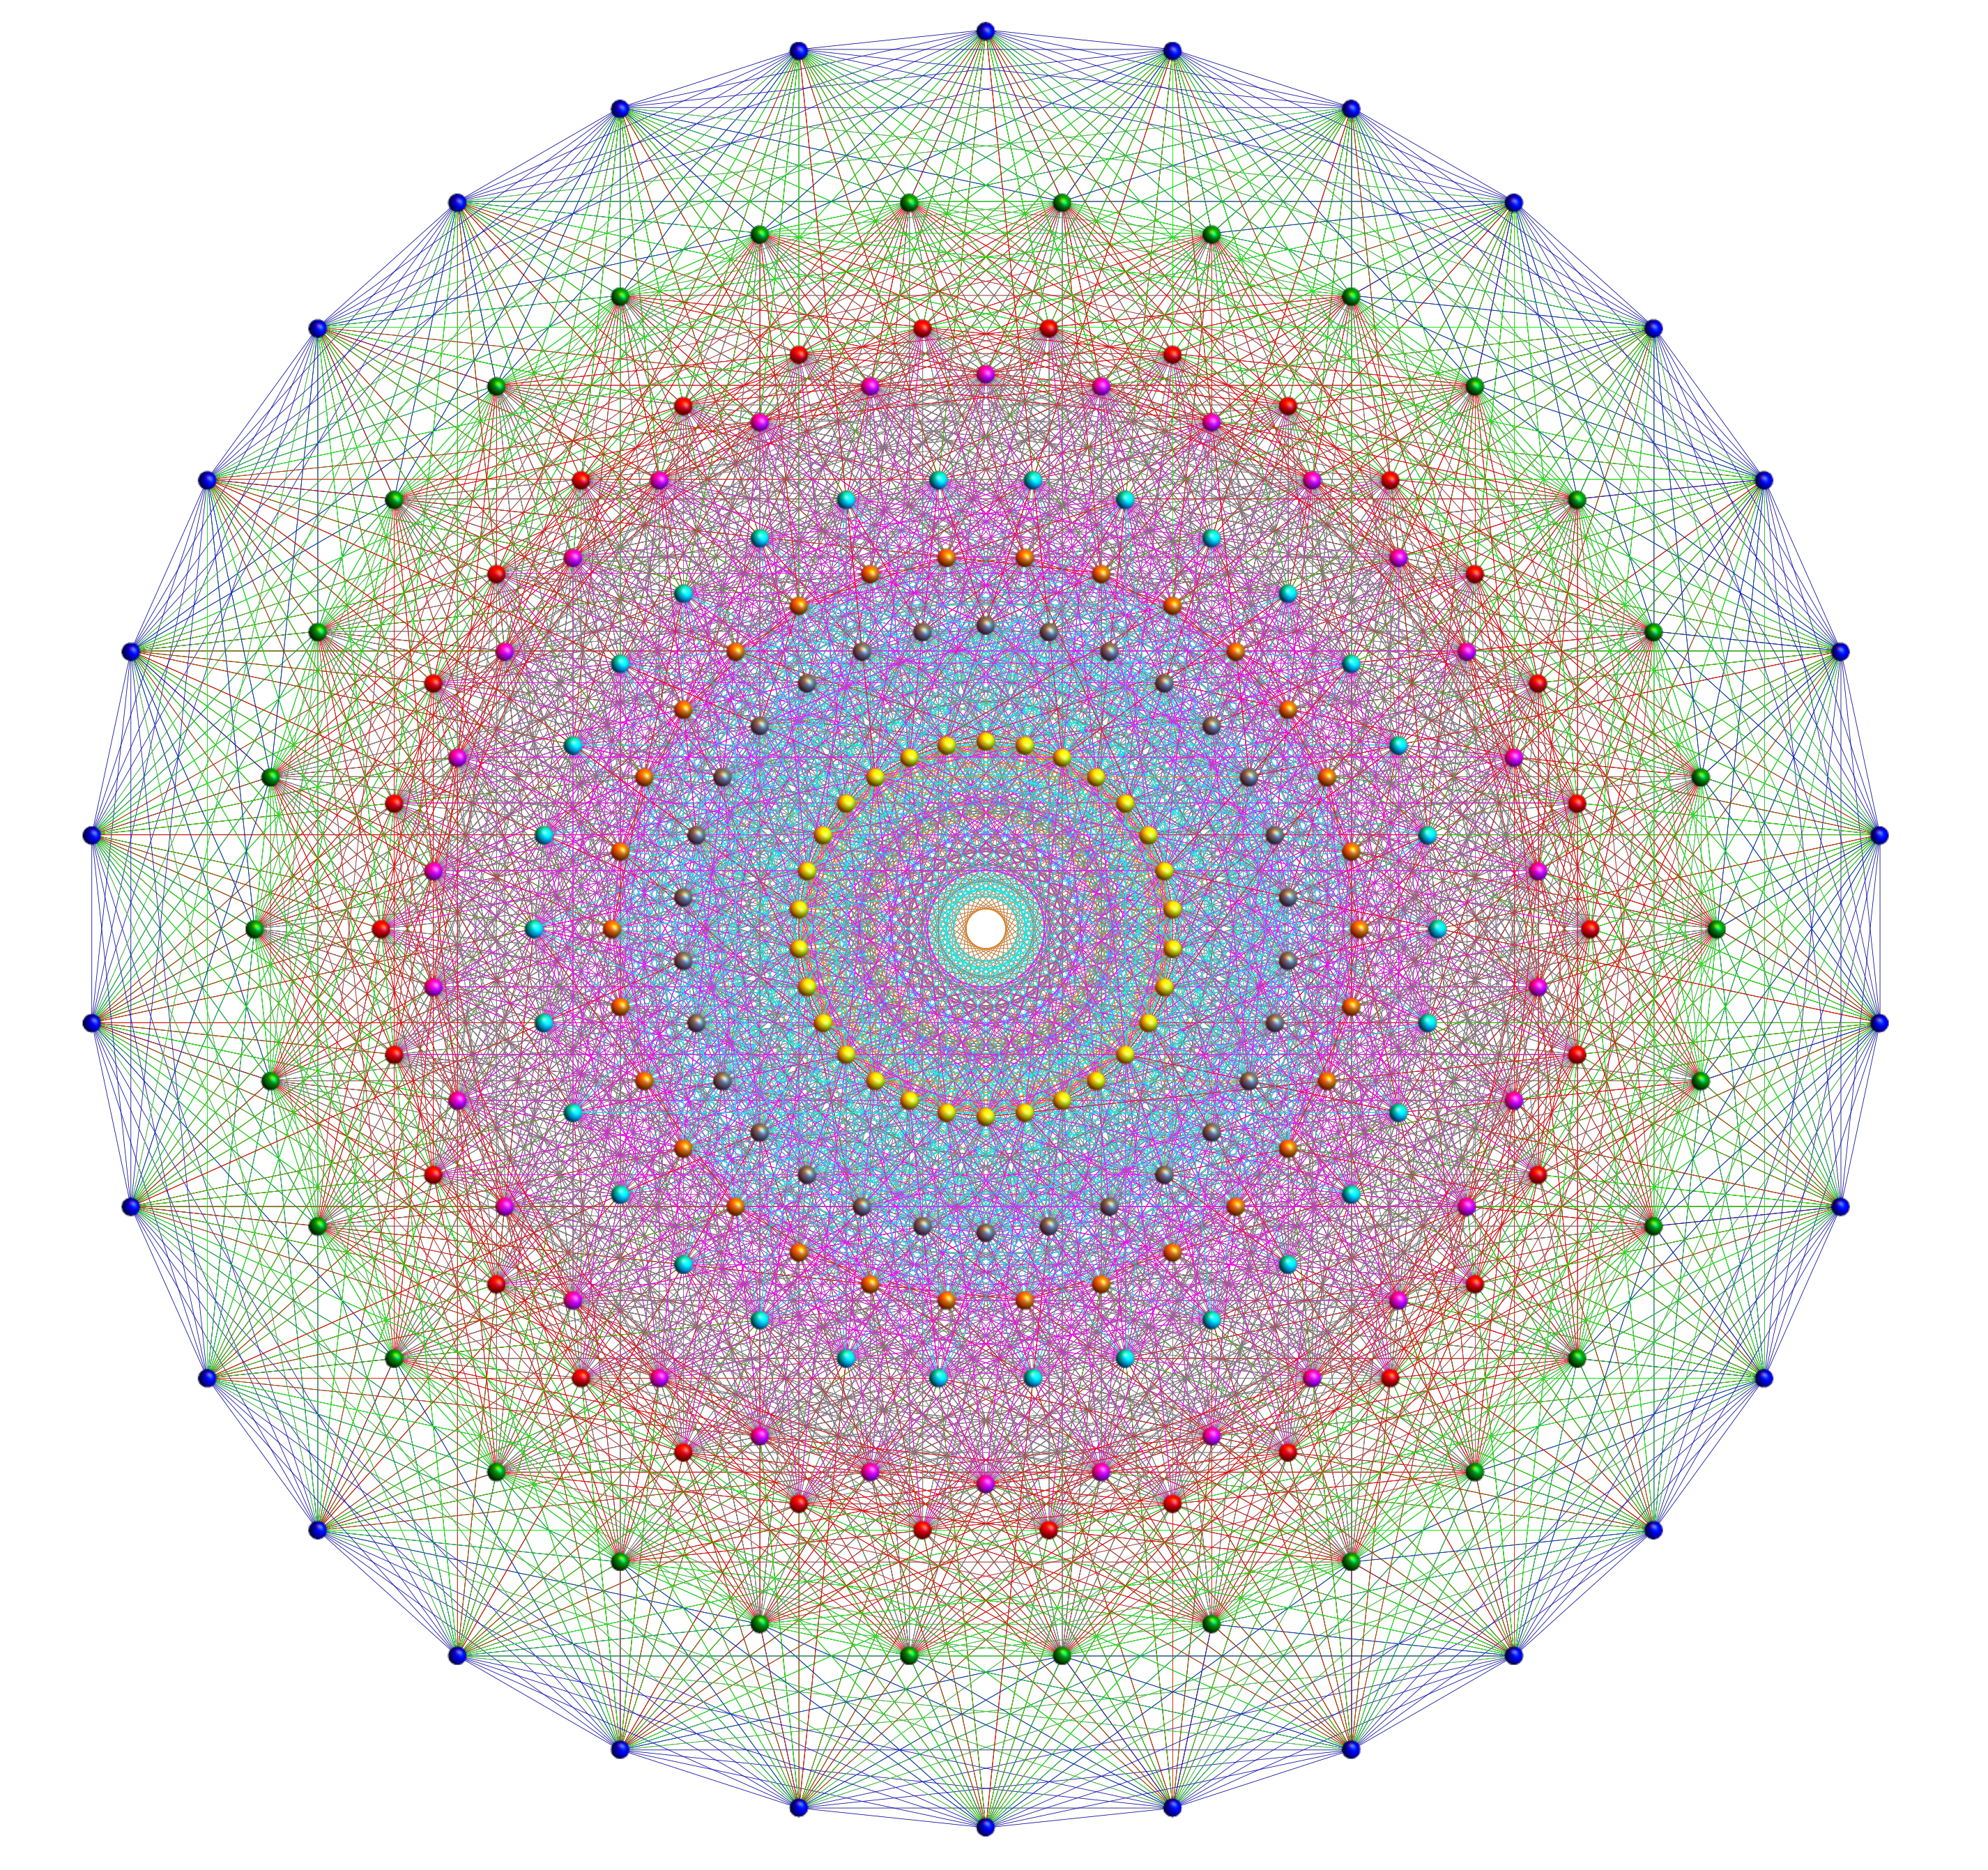
\includegraphics[width=.8\columnwidth]{front.png}
\end{figure}
\newpage
\tableofcontents 
\newpage
\section{Gli interi}
\subsection{Propriet\`a di base}
Una propriet\`a dei numeri interi, che si prender\`a come assiomatica, \`e quella del \textit{buon ordinamento}: 
\begin{center}
	\textit{Ogni insieme non-vuoto di interi maggiori o uguali a $0$, ha un elemento minimo.}
\end{center}
Da questa deriva la seguente.
\begin{teorema}
	{Principio di induzione (prima forma)}{}
	Sia $A(n)$ un'affermazione valida per ogni intero $n\ge 1$. Se
	\begin{enumerate}[(1).]
		\item $A(1)$ \`e vera,
		\item $\forall n \ge  1$, se $A(n)$ \`e vera $\implies A(n+1)$ \`e vera,
	\end{enumerate}
	allora, $\forall n \ge  1$, $A(n)$ \`e vera.
	\begin{proof}
		Sia $S $ l'insieme di interi per cui $A(n)$ \`e falsa. Si mostra che $S$ \`e l'insieme vuoto. 
		Si assume per assurdo che $S\neq \varnothing\Rightarrow \exists n_0 \in S$, con $n_0$ minimo (esistente per il buon ordinamento), e, per assunzione, deve essere $n_0 \neq 1 \Rightarrow  n_0>1$. 
		Questo vuol dire che $n_0 -1$ non \`e in $S$ e, quindi, $A(n_0-1)$ \`e vera.

		Per la propriet\`a (2), per\`o, deve essere vera anche $A(n_0)$ perch\'e $n_0 = (n_0-1) + 1$, il che \`e assurdo e, pertanto, $S = \varnothing$.
	\end{proof}
\end{teorema}

\begin{obs}
	Nella dimostrazione sopra, si sarebbe potuto sostituire $1$ con $0$ e far partire il principio di induzione da $n=0$ piuttosto che da $n=1$ e non sarebbe cambiato nulla.
\end{obs}
\noindent Il principio di induzione pu\`o essere espresso in una forma alternativa, come segue.
\begin{teorema}
	{Principio di induzione (seconda forma)}{}
	Sia $A(n)$ affermazione vera $\forall n\ge 0$ e sia possibile mostrare che:
	\begin{enumerate}[(1').]
		\item $A(0)$ \`e vera;
		\item $\forall n > 0$, se $A(k)$ \`e vera $\forall 0\le k < n$, allora $A(n)$ \`e vera.
	\end{enumerate}
	Allora $A(n)$ \`e vera $\forall n\ge 0$.
	\begin{proof}
	Sia ancora $S$ l'insieme degli interi che non soddisfano $A(n)$. 
	Ancora per assurdo, si prende $S\neq \varnothing$, quindi deve esistere, per il buon ordinamento, un $n_0 \in S$ minimo.

	Per punto (1'), deve valere $n_0 \neq 0$ e, visto che $n_0$ \`e minimo, $\forall k$ intero tale che $0\le k< n_0$, $A(k)$ deve essere vera. 
	Per il punto (2'), per\`o, deve essere vera anche $A(n_0)$, arrivando nuovamente all'assurdo.
	\end{proof}
\end{teorema}
\noindent Un altro importante risultato del buon ordinamento \`e l'\textit{algoritmo di Euclide}.
\begin{teorema}
	{Algoritmo di Euclide}{}
	Siano $m,n$ interi, con $m>0$; allora esistono interi $q,r$, con $0\le r< m$, tali che
	\begin{equation}
		n = qm  + r
	\end{equation}
	Inoltre, gli interi $q,r$ sono univocamente determinati da tali condizioni.
	\begin{proof}
		Visto che l'insieme degli interi $q$ tali per cui $qm\le n$ \`e limitato superiormente per definizione, si pu\`o usare il buon ordinamento per affermare che esiste un elemento pi\`u grande\footnote{Basta applicare il buon ordinamento all'elemento pi\`u piccolo dell'insieme $n-qm$.} tale che
		\[
		qm \le n < (q+1) m = q m + m
		\] 
		ossia $0\le n - qm < m$. Sia $r = n - qm$, per cui vale $0\le r < m$. Questo dimostra l'esistenza di $r,q$ come descritti.

		Per l'unicit\`a, si assume che valga contemporaneamente
		\[
		\begin{cases}
			n = q_1m + r_1&, \ 0\le r_1<m\\
			n = q_2m + r_2&, \ 0\le r_2<m\\
		\end{cases}
		\] 
		con $r_1 \neq r_2$. Sia, per esempio, $r_2> r_1$; allora, sottraendo le due, si ha $(q_1-q_2) m = r_2-r_1$. 
		Per\`o, si ha $r_2-r_1> 0$ e $r_2-r_1 < m$, il che non \`e possibile perch\'e $q_1-q_2$ \`e un intero per cui $(q_1 - q_2)m > 0$, quindi si avrebbe $r_2-r_1 = (q_1-q_2)m \ge m$ e, quindi $r_2-r_1\ge m$.
		Pertanto, deve essere $r_1=r_2$, che fra l'altro implica $q_1m=q_2m$, per cui $q_1=q_2$.
	\end{proof}
\end{teorema}
\noindent Da questo teorema, si definisce $r$ come il \textit{resto della divisione di $n$ per $m$}.
\subsection{Massimo comune divisore}
Siano $n, d$ due interi diversi da $0$.
Si dice che $d$ \textit{divide} $n$ se esiste $q$ intero tale che $n = dq$; in questo caso, si scrive $d|n$.
Se $m,n$ sono interi non-nulli, per \textit{divisore comune} di $m$ e $n$ si intende un intero $d\neq 0$ tale che $d | m$ e $d | n$. 
Allora si ha la seguente definizione.
\begin{definizione}
	{Massimo comune divisore}{}
	Per massimo comune divisore di $m,n$ interi non nulli, si intende un intero $d>0$, divisore comune di $m$ e $n$, e tale che $\forall e $ intero positivo che divide $m$ e $n$, si ha anche $e|d$.
\end{definizione}
\noindent Chiaramente, il massimo comune divisore \`e univocamente determinato e si mostrer\`a che esiste sempre. 
Per farlo, si d\`a prima la seguente definizione.
\begin{definizione}
	{Ideale}{}
	Sia $J\subseteq \mathbb{Z}$ un sottoinsieme degli interi. Si dice che $J$ \`e un \textit{ideale} se:
	\begin{itemize}
		\item $0 \in J$;
		\item $m,n\in J\implies m+n \in J$
		\item se $m\in J$ e $n$ \`e un intero qualsiasi, allora $mn \in J$.
	\end{itemize}
\end{definizione}
\begin{obs}
	Di seguito, per ideale si intender\`a sempre un sottoinsieme degli interi.
\end{obs}
\noindent Siano $m_1, \ldots,m_r$ interi. Sia $J$ l'insieme di tutti gli interi che si scrivono come
\[
x_1m_1+\ldots+x_r m_r
\] 
con $x_1,\ldots,x_r$ interi. 
Allora \`e automaticamente verificato che $J$ \`e un ideale. Infatti
\begin{itemize}
	\item se $y_1,\ldots,y_r$ sono interi, allora
		\[
		\sum_{i=1}^{r} x_i m_i +  \sum_{j=1}^{r} y_j m_j = (x_1 + y_1) m_1 + \ldots + (x_r + y_r) m_r
		\] 
		che, quindi, appartiene a $J$;
	\item se $n$ \`e un intero, si ha
		\[
		n \sum_{i=1}^{r} x_i m_i = nx_1m_1 + \ldots+ nx_r m_r
		\] 
		che, quindi, appartiene a $J$;
	\item si pu\`o scrivere $0$ come $0m_1 + \ldots + 0m_r$, quindi anche $0 \in J$.
\end{itemize}
In questo caso, si dice che $J$ \`e \textbf{generato} dagli interi $m_1,\ldots,m_r$ e che questi sono i suoi \textbf{generatori}. L'insieme $\left\{ 0 \right\} $ \`e esso stesso un ideale, chiamato \textbf{ideale nullo}. 
Inoltre, $\mathbb{Z}$ \`e detto \textbf{ideale unit\`a}.
Ora si pu\`o dimostrare il seguente.
\begin{teorema}
	{}{smalld}
	Sia $J$ un ideale di $\mathbb{Z}$. Allora esiste un intero $d$ che \`e un generatore di $J$. Inoltre, se $J \neq \left\{ 0 \right\} $, allora $d$ \`e il pi\`u piccolo intero positivo in $J$.
	\begin{proof}
	Sia $J$ l'ideale nullo; allora $0$ \`e un suo generatore.
	Sia, ora, $J \neq \left\{ 0 \right\} $; se $n \in J$, allora $-n = (-1) n $ \`e anche in $J$, quindi $J$ contiene degli interi positivi.
	Si vuole dimostrare che $d$, definito come il pi\`u piccolo intero positivo, \`e un generatore.
	Per farlo, sia $n \in J$, con $n = dq + r, \ 0\le  r < d$; allora $r = n - dq \in J$ e, visto che vale $r < d$, segue che $r = 0$\footnote{Altrimenti $d$ non sarebbe il pi\`u piccolo intero positivo.}, quindi $n = dq$ e, allora, $d$ \`e un generatore.
	\end{proof}
\end{teorema}
\begin{teorema}
	{}{bezid}
	Siano $m_1,m_2$ due interi positivi e sia $d$ un generatore positivo per l'ideale generato da $m_1,m_2$. Allora $d$ \`e il massimo comune divisore di $m_1,m_2$.
	\begin{proof}
		Per definizione, $m_1,m_2 \in J$\footnote{Questo \`e ovvio perch\'e $m_1 = 1m_1 + 0 m_2$ e $m_2  = 0 m_1 + 1 m_2$.}, quindi esiste un intero $q_1$ tale che $m_1=q_1 d$, per cui $d|
		m_1$.
		Analogamente $d|m_2$.
		Sia, poi, $e$ un intero non-nullo che divide sia $m_1$ che $m_2$ come $m_1 = h_1 e$ e $mm_2=h_2 e$, con interi $h_1,h_2$.
		Visto che $d$ \`e nell'ideale generato da $m_1,m_2$, esistono degli interi $s_1,s_2$ tali che $d = s_1m_1 + s_2m_2$, quindi
		\[
		d = s_1h_1e + s_2h_2e = (s_1h_1 + s_2h_2) e
		\] 
		Quindi $e $ divide $d$ e il teorema \`e dimostrato.
	\end{proof}
\end{teorema}
\begin{obs}
	La stessa esatta dimostrazione funziona per pi\`u di due interi, quindi se si considerassero $m_1,\ldots,m _r$ degli interi, con $d$ generatore positivo dell'ideale da loro generato, $d$ sarebbe anche il massimo comune divisore.
\end{obs}
\noindent Questi due teoremi permettono di concludere i seguenti fatti.
\begin{itemize}
	\item Ogni ideale $J$ contiene un numero intero che lo genera interamente e questo coincide col pi\`u piccolo intero positivo in esso contenuto, quindi \`e l'unico generatore \textit{singolo} dell'ideale.
	\item Ogni insieme di numeri interi ha un massimo comune divisore perch\'e tale insieme genera un ideale, il quale, per\`o, contiene un generatore (pi\`u piccolo numero intero in esso contenuto) che \`e un massimo comune divisore per l'insieme di interi iniziale.
\end{itemize}
\begin{definizione}
	{Interi coprimi}{relprime}
	Siano $m_1,\ldots,m_r$ degli interi il cui massimo comune divisore \`e $1$. 
	Allora $m_1,\ldots,m_r$ si dicono \textit{coprimi} e, per questi, esistono interi $x_1,\ldots,x_r$ tali che
	\[
	x_1m_1   +\ldots + x_r m_r = 1
	\] 
	perch\'e $1$ appartiene all'ideale generato dagli $m_i$.
\end{definizione}
\`E immediato verificare per definizione di ideale che $1 \in  J \iff J \equiv \mathbb{Z}$.
Dalla definizione \ref{def:relprime} segue direttamente che ogni insieme di interi coprimi genera $\mathbb{Z}$.
\begin{obs}
	Si potrebbe pensare che se $p$ \`e un numero primo, allora l'insieme $\left\{ p \right\} $ generi $\mathbb{Z}$, cio\`e $p$ generi $\mathbb{Z}$. 
	Questo \`e ovviamente falso sia perch\'e, evidentemente, $J_p$ non contiene $1$, sia perch\'e $p$ non \`e coprimo con se stesso, avendo come altro divisore proprio $p$ oltre che $1$.
\end{obs}
\subsection{Fattorizzazione unica}
\begin{definizione}
	{Numero primo}{}
	Si dice che $p$ \`e un numero primo se \`e un intero e $p\ge   2$ tale che, data una fattorizzazione $p = mn $, con interi positivi $m,n$, allora $m=1$ o $n=1$.
\end{definizione}
\begin{obs}
	Il fatto che $p=mn$ con $m=1$, o $n=1$ implica $p$ numero primo significa che $p$ \`e diviso unicamente o da $1$ o, da se stesso.
\end{obs}
\noindent Ora si mostra che ogni numero intero ammette un'unica scomposizione in numeri primi. 
Per dimostrare l'unicit\`a di tale scomposizione, si introduce il seguente lemma.
\begin{lemma}
	{}{lemmaprimdecomp}
	Sia $p$ un numero primo e siano $m,n$ interi non-nulli e tali che $p$ divide $mn$. Allora o $p|m$ o $p |n$.
	\begin{proof}
		Senza perdita di generalit\`a, si assume che $p$ \textit{non} divida $m$. 
		Allora, il massimo comune divisore di $p$ e $m$ deve essere $1$, pertanto esistono interi $a,b$ tali per cui $1 = ap + bm$.

		Ora, moltiplicando ambo i membri per $n$, si ha $n = nap + bmn$, ma $mn = pc$ per qualche intero $c$ (essendo in assunzione $mn$ divisibile per $p$), quindi
		\[
		n = nap + bpc = (na + bc) p
		\] 
		il che implica che $p$ divide $n$.
	\end{proof}
\end{lemma}
\noindent Per evidenziare l'utilit\`a del lemma nel seguente teorema, si nota che se $p$ divide un prodotto di numeri primi $q_1\ldots q_s$, si hanno due possibilit\`a: o $p$ divide $q_1$, o divide $q_2 \ldots q_s$; se divide $q_1$, allora $p \equiv q_1$, altrimenti si trova $p\equiv q_i$ procedendo induttivamente. 
Il caso interessante \`e quando si ha un uguaglianza tra prodotti di numeri primi 
\[
p_1 \ldots p_r = q_1\ldots q_s
\] 
dove ogni $p_i$ divide il prodotto\footnote{Per vederlo, \`e sufficiente prendere $c = p_1 \ldots p_{i-1} p_{i+1} \ldots p_r$, quindi si ha $c p_i = q_1 \ldots q_s$, che \`e la definizione di $p_i | q_1 \ldots q_s$.}. Rinumerandoli, si pu\`o assumere senza perdita di generalit\`a che $p_1 = q_1$ e, induttivamente, che $p_i = q_i$ e $r = s$, essendo due scomposizioni in un numeri primi.
\begin{teorema}
	{}{}
	Ogni intero positivo $n\ge   2$ ammette una fattorizzazione come prodotto di numeri primi (non necessariamente distinti) $n=p_1\ldots p_r$ e tale fattorizzazione \`e unica.
	\begin{proof}
		Si assume per assurdo che esista almeno un intero $\ge  2 $ che non possa essere espresso come prodotto di numeri primi.
		Sia $m$ il pi\`u piccolo di questi. 

		Per costruzione, $m$ non pu\`o essere primo, quindi $m = de$, con $d,e > 1$. 
		Visto che $d$ ed $e$ sono minori di $m$ e visto che $m$ \`e scelto per essere il pi\`u piccolo fra gli interi non fattorizzabili come numeri primi, allora sia $d$ che $e$ ammettono scomposizione in prodotto di numeri primi:
		\[
		\begin{split}
			&d = p_1 \ldots p_r \\
			&e = p'_1 \ldots p'_s
		\end{split}\implies m = p_1 \ldots p_r p'_1 \ldots p'_s
		\] 
	da cui l'assurdo.	

	Per mostrare l'unicit\`a, si usa il lemma \ref{lem:lemmaprimdecomp}. 
	Come conseguenza, diretta del lemma, se esistessero due scomposizioni in primi $p_1 \ldots p_r $ e $p'_1 \ldots p'_s$, varrebbe $p_1 \ldots p_r = p'_1 \ldots p'_s\Rightarrow p_i = p'_i$ e $r = s$, da cui l'unicit\`a
	\end{proof}
\end{teorema}
\subsection{Identit\`a di B\'ezout e equazioni diofantee}

\subsubsection{Identit\`a di B\'ezout}
L'identit\`a di B\'ezout non \`e altro che quanto espresso in teorema \ref{th:bezid}. Di seguito lo si enuncia senza ricorrere a tale trattazione. 
\begin{teorema}
	{Identit\`a di B\'ezout}{}
	Dati $a,b \in \mathbb{Z}$ non entrambi nulli, esistono altri due interi $m,n$ tali che:
	\[
	\operatorname{gcd} (a,b) = am +  bn
	\] 
\begin{proof}
	Si considera l'insieme di tutte le possibili combinazioni lineari positive di $a,b$, dato da $\mathrm{CL} ^+(a,b) : = \left\{ ar+ bs : r, s \in \mathbb{Z} , \ ar + bs > 0 \right\} $. Questo \`e non-vuoto perch\'e, assumendo senza perdita di generalit\`a $a\neq 0$, esistono, per $s =0 $, degli $r\in \mathbb{Z}$ tali che $ra >0 $.

	Visto che $\mathrm{CL} ^+(a,b) \subseteq \mathbb{N}$, per il principio del buon ordinamento, questo ammette un minimo $d$; in quanto tale $\exists m,n \in \mathbb{Z}:d = am + bn$. 
	Infine, si motra che $d = \operatorname{gcd} (a,b)$, cio\`e si mostrano i seguenti punti.
	\begin{itemize}
		\item Si ha $d|a$ e $d|b$.

			Dividendo $a$ per $d$, si ha $a = qd +r$, con $0\le r < d$, quindi
			\[
			a = q ( am +  bn) + r
			\] 
			da cui 
			\[
			r = (-qm + 1) a + (-qn) b
			\] 
			In questo modo, $r$ \`e combinazione lineare di $a,b$ ed \`e minore di $d$, ma questo \`e assurdo perch\'e $d $ era minimo per assunzione, quindi deve essere $r= 0$. Allo stesso modo si mostra $d | b$.
		\item Se $c|a$ e $c|b \implies c \le d$.

			Questo \`e vero perch\'e se $c|a, \ c|b$, allora (in particolare) $c | (am + bn) $, cio\`e $ c | d \Rightarrow c\le d$.
	\end{itemize}
\end{proof}
\end{teorema}
\begin{obs}
	Il teorema afferma l'esistenza di una possibile coppia $(m,n) \in \mathbb{Z} \times \mathbb{Z}$ che soddisfa $\operatorname{gcd} (a,b) = am + bn$, ma non ne specifica l'unicit\`a; di fatto, si vedr\`a che di coppie simili ce ne sono infinite.
\end{obs}
\begin{corollario}
	{}{}
	Dati $a,b \in \mathbb{Z}$ non entrambi nulli e sia $c\in \mathbb{Z} : c|a$ e $c|b$; allora $c | \operatorname{gcd}(a,b) $. 
\end{corollario}
Complessivamente, esattamente come riportato nel teorema \ref{th:bezid}, si \`e dimostrato che il massimo comune divisore di due interi $a,b$ \`e la pi\`u piccola combinazione lineare positiva ottenibile dai due.
\begin{corollario}
	{}{c1}
	Dati $a,b$ non entrambi nulli e $\operatorname{gcd}(a,b) $ il loro massimo comune divsore, allora gli interi 
	\[
		a' = \frac{a}{\operatorname{gcd}(a,b) } \hspace{2cm} b' = \frac{b}{\operatorname{gcd}(a,b) }
	\] 
	sono coprimi.
	\begin{proof}
	Si pu\`o dimostrare in due modi diversi. Nel primo, si assume per assurdo che esista un divisore comune $d> 1 $ di $a' , b'$; se cos\`i fosse, per\`o, $d \cdot \operatorname{gcd}(a,b) $ dividerebbe sia $a$ che $b$ e sarebbe pi\`u grande di $\operatorname{gcd}(a,b) $ stesso, il che \`e assurdo.

	Il secondo fa uso dell'identit\`a di B\'ezout per cui $\operatorname{gcd}(a,b) = am+bn $; dividendo per $\operatorname{gcd}(a,b) $, si ha:
	\[
	1 = a'm + b'n 
	\] 
	per cui $1$ \`e il pi\`u piccolo intero positivo  ottenibile come combinazione lineare positiva di $a', b'$, quindi i due sono coprimi.
	\end{proof}
\end{corollario}
\begin{teorema}
	{}{d1}
	Siano $a,b,c \in \mathbb{Z}$; se $a|bc$ e $\operatorname{gcd}(a,b) =1$, allora $a|c$.
	\begin{proof}
		Per B\'ezout, visto che $\operatorname{gcd}(a,b) = 1$, si ha $1 = an + bm$ per una coppia di numeri $m,n \in \mathbb{Z}$. 
		Moltiplicando ambo i membri per $c$, ne segue che:
		\[
		c = acn + bcm
		\] 
		quindi $a | c$ perch\'e, ovviamente, $a | acn$, mentre $a | bcm$ perch\'e, per ipotesi, $a | bc$, quindi $a| (acn + bcm)$, cio\`e $a | c$.
	\end{proof}
\end{teorema}
\noindent Il teorema appena dimostrato \`e alla base del fatto che la fattorizzazione di interi in numeri primi \`e unica.

\subsubsection{Equazioni diofantee}


Dati $a,b,c \in \mathbb{Z}$, si dice \textbf{equazione diofantea} un'equazione del tipo	
\begin{equation}
	ax + by = c
\end{equation}
La sua soluzione \`e una coppia di interi $(\overline{x},\overline{y}) \in \mathbb{Z} \times \mathbb{Z}$ che la soddisfa.

\begin{obs}
	L'equazione diofantea con $a=b=0$ ha soluzione $\iff c= 0$ e ne ammette infinite, consistenti in tutte le possibili coppie $(\overline{x},\overline{y}) \in \mathbb{Z}\times \mathbb{Z}$, perch\'e ogni coppia soddisfa $0 x + 0y = c$.
\end{obs}
Per il caso generale di $a,b$ non entrambi nulli, si ha il seguente.
\begin{teorema}
	{}{solco}
	L'equazione $ax + by = c$, con $a,b$ non entrambi nulli, ha soluzione $\iff \operatorname{gcd} (a,b )  | c$.
	\begin{proof}
		Per l'identit\`a di B\'ezout, si sa che vi \`e soluzione all'equazione 
		\[
		ax + by = \operatorname{gcd}(a,b) 
		\] 
		L'equazione da risolvere \`e diversa: al posto di $\operatorname{gcd}(a,b) $ c'\`e $c$; allora la dimostrazione si basa sul capire se $\operatorname{gcd}(a,b) $ divide o meno $c$.

		Nel caso in cui $\operatorname{gcd}(a,b) | c$ (per cui si ha $c = k\cdot \operatorname{gcd}(a,b) $ per qualche intero $k$), allora l'equazione diofantea ammette soluzione. Infatti, dopo aver trovato $(m,n) \in \mathbb{Z} \times \mathbb{Z}$ che risolve $am + bn = \operatorname{gcd}(a,b) $, si ha che $(m k , nk) \in \mathbb{Z} \times \mathbb{Z}$ risolve l'equazione diofantea perch\'e 
		\[
		k \cdot (am + bn ) = akm + bkn = k\cdot \operatorname{gcd}(a,b) = c
		\] 
		Viceversa, se $\operatorname{gcd}(a,b)$ non divide $c$, allora non vi \`e soluzione. Se, per assurdo, vi fosse soluzione, sia questa $(\overline{x},\overline{y})$, allora $a \overline{x}+ b \overline{y}=c$ implica che $\operatorname{gcd}(a,b) | c$ perch\'e $\operatorname{gcd}(a,b) $ divide il membro di sinistra (essendo un divisore sia di $a$ che di $b$). 
		Questo, per\`o, \`e assurdo perch\'e si era nell'ipotesi in cui $\operatorname{gcd}(a,b) \not | \ c$.
	\end{proof}
\end{teorema}
Si considera il caso in cui l'equazione $ax + by = c$ ha soluzione; si vuole capire se la soluzione \`e unica, o se ve ne sono di pi\`u. 
Si considera, a tal proposito, l'\textbf{omogenea associata} $ax + by = 0$. 
\begin{obs}
	La comodit\`a nel lavorare con l'omogenea associata sta nel fatto che se $(\overline{x}, \overline{y})$ risolve $ax + by = c$ e  $(\gamma, \delta )$ risolve l'omogenea, allora $(\overline{x}+\gamma, \overline{y}+\delta )$ \`e ancora soluzione di $ax + by = c$.
\end{obs}
\noindent L'obiettivo, ora, \`e di trovare il numero delle soluzioni per l'omogenea associata.
Si nota che $ax + by =0 \Rightarrow  axa = - by$; si risolve
\[
\frac{a}{\operatorname{gcd}(a,b) } x = - \frac{b}{\operatorname{gcd}(a,b) } y 
\] 
Sia $(\gamma, \delta )$ una soluzione di questa; visto che $a/\operatorname{gcd}(a,b) $ e $b / \operatorname{gcd}(a,b) $ sono coprimi\footnote{Vedi corollario \ref{cor:c1}.}, il teorema \ref{th:d1} afferma che $a / \operatorname{gcd}(a,b) $ divide $\delta $, quindi $\delta $ \`e della forma $\frac{a}{\operatorname{gcd}(a,b)}  t$ e $\gamma$, analogamente, \`e della forma $- \frac{b}{\operatorname{gcd}(a,b)} t$.

Al contrario, si nota facilmente che una qualunque coppia della forma $\left( - \frac{b}{\operatorname{gcd}(a,b) }t , \frac{a}{\operatorname{gcd}(a,b) }t\right)$, con $ t \in \mathbb{Z} $ \`e una soluzione dell'omogenea associata. 
Questo significa che le soluzioni dell'omogenea associata sono tutte di questa forma, pertanto sono infinite.

Da questo discorso, si pu\`o concludere che anche le soluzioni dell'equazione diofantea iniziale $ax + by = c$ sono infinite. 
Il teorema di seguito permette di concludere, ulteriormente, che \textit{tutte} le soluzioni di $ax + by = c$ sono esprimibili tramite quelle dell'omogenea, quindi equazione originale e omogenea hanno lo stesso numero di soluzioni.
\begin{teorema}
	{}{}
	Se l'equazione $ax + by = c$ ammette soluzione, allora ne ammette infinite. Data $(\overline{x}, \overline{y})$ una sua soluzione, l'insieme $\mathcal{S} $ di tutte le soluzioni di $ax +by = c$ \`e ottenibile come
	\[
	\mathcal{S}  = \left\{ (\overline{x}+\gamma, \overline{y}+\delta ) : (\gamma, \delta ) \text{ soluzione dell'omogenea associata}\right\} 
	\] 
	\begin{proof}
		Per quanto detto sopra, si conclude che 
		\[
		\left\{(\overline{x}+\gamma, \overline{y}+\delta ) : (\gamma, \delta ) \text{ soluzione dell'omogenea associata}  \right\} \subseteq \mathcal{S} 
		\] 
		Si deve mostrare l'inclusione inversa.
		Questo segue direttamente dal fatto che, se $(\alpha ,\beta )$ \`e soluzione di $ax + by = c$, allora $(\alpha -\overline{x}, \beta - \overline{y})$ \`e soluzione dell'omogenea associata.
	\end{proof}
\end{teorema}



\subsection{Relazioni di equivalenza e congruenza}
\begin{definizione}
	{Relazione di equivalenza}{}
	Sia $S$ un insieme.
	Una relazione di equivalenza su $S$ \`e una relazione indicata con $x \sim y, \ x, y \in S$, tale che:
	\begin{enumerate}[ER 1.]
		\item $\forall x \in S, \ x \sim x$;
		\item se $x \sim y$ e $y\sim z$, allora $x \sim z$;
		\item se $x\sim y$, allora $y \sim x$.
	\end{enumerate}
\end{definizione}
\noindent Se su $S$ \`e definita una relazione di equivalenza $\sim$, le classi di equivalenza sono insiemi $C_x : = \left\{ y \in S : y \sim x \right\} $ partizionano $S$ in insiemi disgiunti. 
Inoltre, dati due elementi $r,s \in S$, si ha $C_r \equiv C_s$, oppure $C_r,\ C_s$ non hanno elementi in comune.
Si sceglie un elemento che identifica la classe di equivalenza, ad esempio $x$ per $C_x$, e tale elemento si chiama rappresentante della classe di equivalenza. 
Un esempio di relazione di equivalenza \`e la congruenza.
\begin{definizione}
	{Congruenza}{}
	Sia $m \in \mathbb{Z}^+$ e $a,b \in \mathbb{Z}$; si dice che $a$ \`e \textit{congruente} $b$ \textit{modulo} $m$ se $\exists k \in \mathbb{Z} : a-b = km$. In tal caso, si scriver\`a $a \equiv b  \pmod{m}  $.
\end{definizione}
\begin{obs}
	La definizione pi\`u esplicativa di congruenza \`e che due numeri $a,b \in \mathbb{Z}$ di dicono congruenti modulo $m \in \mathbb{Z}^+$ se, divisi per $m$, restituiscono lo stesso resto.
	Di fatto, da questa discende la definizione data sopra: se $a = qm + r, \ b = pm + r \Rightarrow a - b = (q-p)m$.
\end{obs}
\begin{definizione}
	{Interi pari e dispari}{}
Si definiscono gli interi \textbf{pari} come quelli che sono congruenti a $0 \pmod{2} $ (quindi $n = 2m$) e quelli \textbf{dispari} come gli interi che non sono pari, quindi della forma $2m + 1$, per qualche intero $m$.
\end{definizione}
\noindent Dalla definizione di congruenza, si ha che $a\equiv b \pmod{m}  \Rightarrow  a- b = qm$, quindi $a-b$ appartiene all'ideale generato da $m$.

Inoltre, la stessa relazione implica che $m | (a-b)$; viceversa, se $a \not \equiv b \pmod{m} $, allora i due numeri divisi per $m$ avrebbero resti diversi: $a = k_1 m + r_a, \ b = k_2 m + r_b$, il che implica che $a-b = (k_1 - k_2)m + (r_a- r_b)$, che non \`e divisibile per $m$; allora is ha il seguente.
\begin{prop}
	{}{}
	Siano $m \in \mathbb{Z}^+$ e $a,b \in \mathbb{Z}$; $a$ e $b$ sono congruenti se e soltanto se $m | (a-b)$.
\end{prop}
\begin{prop}
	{Addizione e moltiplicazione in congruenza}{}
	Dati $a\equiv a' \pmod{m} $ e $b\equiv b' \pmod{m} $, si ha:
	\[
		\begin{split}
			&a + b \equiv a' + b' \pmod{m}  \\
			& a b\equiv a'b' \pmod{m} 
		\end{split}
	\] 
\begin{proof}
	Per definizione, si ha $a ' = a + km$ e $b' = b + k'm $; quindi:
	\[
	a' + b ' = a+ b + (k+k') m\implies a' + b' \equiv a + b\pmod{m} 
	\] 
	Per la moltiplicazione, si nota che 
	\[
	a' b ' = a b + m(kb + k'a) +kk'm^2
	\] 
	da cui si vede che $a'b' - ab$ \`e divisibile per $m$, quindi $a'b' \equiv ab \pmod{m} $.
\end{proof}	
\end{prop}
La divisione in congruenza funziona diversamente; infatti $2 \cdot  7 \equiv 2 \cdot  4 \pmod{6} $, ma $7 \not \equiv 4 \pmod{6} $. 
Si ha il seguente.
\begin{teorema}
	{Divisione in congruenza}{}
	Sia $m \in \mathbb{Z}^+$; $\forall a \in  \mathbb{Z} \setminus \left\{ 0 \right\} $ e dati $b_1,b_2 \in \mathbb{Z}$, vale
	\[
	ab_1 \equiv ab_2 \pmod{m} \iff b_1 \equiv b_2 \mod{\frac{m}{\operatorname{gcd}(a,m) }} 
	\] 
	Questo vuol dire che la divisione \`e ammessa a patto di dividere il modulo per $\operatorname{gcd}(a,m) $.
	\begin{proof}
		Si mostra l'implicazione verso destra.
		Per definizione, $m  \mid  (ab_1- ab_2)$, quindi $\exists q \in \mathbb{Z} : mq = ab_1 - ab_2$.
		Dividendo per $\operatorname{gcd}(a,m) $:
		\[
		\frac{a}{\operatorname{gcd}(a,m) } (b_1-b_2) = \frac{m}{\operatorname{gcd}(a,m) } q
		\] 
		Ma $a / \operatorname{gcd}(a,m) $ e $m / \operatorname{gcd}(a,m) $ sono coprimi, quindi $\big(m / \operatorname{gcd}(a,m) \big)  \mid (b_1-b_2)$, il che implica che
		\[
		b_1\equiv b_2 \mod \frac{m}{\operatorname{gcd}(a,m) }
		\] 
		Per l'implicazione inversa, si assume che
		\[
		b_1\equiv b_2 \mod \frac{m}{\operatorname{gcd}(a,m) }
		\] 
		per cui $\exists t \in \mathbb{Z}$ tale che 
		\[
		t \frac{m}{\operatorname{gcd}(a,m) } = b_1-b_2 \implies tm  = (b_1-b_2) \operatorname{gcd}(a,m) 
		\] 
		quindi $m  \mid (b_1 -b_2) \operatorname{gcd}(a,m) $. 
		Usando che $\operatorname{gcd}(a,m) | a$, si ottiene che
		\[
		m | (b_1-b_2) a \implies ab_1 \equiv ab_2 \pmod{m} 
		\] 
	\end{proof}
\end{teorema}
\subsubsection{Inversi in congruenze}
Gli unici inversi moltiplicativi in $\mathbb{Z}$ sono $+1, -1$; operando con le congruenze, si riescono a trovare altri inversi moltiplicativi a patto di definire correttamente cosa vuol dire.
\begin{definizione}
	{Inverso in congruenza}{}
	Sia $m \in  \mathbb{Z}^+$; l'inverso di $a \in \mathbb{Z}$ \`e un certo $e \in \mathbb{Z}$ tale che
	\[
	e \cdot  a \equiv 1 \pmod{m} 
	\] 
\end{definizione}
\begin{esempio}
Per esempio, $2$ \`e l'inverso di $3 \operatorname{mod} 5$ perch\'e $2 \cdot 3 = 6 \equiv 1 \pmod{5} $.
\end{esempio}
\begin{obs}
	Quando un numero ammette inverso in congruenza, ne ammette infiniti; infatti, se $a$ \`e l'inverso di $n \operatorname{mod} m$, allora
	\[
	n \cdot  ( a+km ) \equiv n\cdot a + knm \equiv 1 + knm \equiv 1 \pmod{m} 
	\] 
\end{obs}
Non sempre un numero ammette un inverso moltiplicativo per qualche modulo; di seguito, \`e riportata una condizione necessaria e sufficiente per l'esistenza dell'inverso.
\begin{teorema}
	{}{}
	Un numero $a \in \mathbb{Z}$ ha inverso $\operatorname{mod} m $ se e solo se $\operatorname{gcd}(a,m) = 1$.
	\begin{proof}
		Si assume che $\operatorname{gcd}(a,m) =1 $; per B\'ezout, si ha:
		\[
		a u + m v = 1 
		\] 
		per qualche coppia $u,v \in \mathbb{Z}$. 
		Questa uguaglianza, letta modulo $m$, diventa:
		\[
		a u \equiv 1 \pmod{m} 
		\] 
		cio\`e $u$ \`e inverso di $a \operatorname{mod}m  $.

		Per l'implicazione inversa, si assume che $a$ abbia inverso moltiplicativo $u$.
		Questo implica che $au \equiv 1 \pmod{m} $, che, a sua volta, diventa:
		\[
		a u - mk =1
		\] 
		per qualche $k \in \mathbb{Z}$. 
		Questo \`e sufficiente per affermare che $\operatorname{gcd}(a,m) =1$. 
	\end{proof}
\end{teorema}

\subsubsection{Congruenze lineari in una incognita}
Si cercano le soluzioni $x$ alla congruenza $ax \equiv b \pmod{m} $. 
Si inizia col notare che se $\exists d \in \mathbb{Z}$ tale che $d | a$ e $d | m$, ma $d \not  \mid  b$ allora l'equazione non ha soluzioni.
\begin{proof}
	Se per assurdo ne avesse almeno una $\overline{x}$, allora sarebbe soddisfatta $a \overline{x} - b = q m $, per qualche $q \in \mathbb{Z}$. 
	Ma, nonostante $m$ sia divisibile per $d$, l'altro membro non risulta tale per via di $b$, il che \`e assurdo. 
\end{proof}
Da quanto appena notato, si conclude la condizione necessaria perch\'e esista almeno una soluzione, ossia $\operatorname{gcd}(a,m) | b$.
\begin{obs}
	Se $k | a,b$, allora l'equazionoe 
	\[
	\frac{a}{k} x \equiv \frac{b}{k} \mod \frac{m}{\operatorname{gcd}(k,m) }
	\] 
	\`e equivalente a $a x \equiv b \pmod{m} $, cio\`e hanno le stesse soluzioni. 
	Si nota in particolare che, se $s$ \`e un numero primo, allora l'equazione $sax \equiv sb \pmod{m} $ ha stesse soluzioni di quella di partenza.
\end{obs}
\begin{teorema}
	{}{}
	La congruenza $ax \equiv b \pmod{m} $ ha soluzione se e soltanto se $\operatorname{gcd}(a,m) | b$. 
	Inoltre, il numero totale di soluzioni \`e $\operatorname{gcd}(a,m) $: le altre si ottengono sommandogli un multiplo di $m$.
	\begin{proof}
		La prima parte si \`e gi\`a dimostrata, quindi si dimostra solo quella relativa al numero di soluzioni.
		Assumendo che effettivamente $\operatorname{gcd}(a,m) | b$, allora $\operatorname{gcd}(a,m) $ \`e il massimo divisore comune di $a,b,m$; allora, dividendo la congruenza per questo, si ha:
		\[
		a' x \equiv b ' \pmod{m'} 
		\] 
		dove 
		\[
		a' = \frac{a}{\operatorname{gcd}(a,m) }\hspace{1cm} b' = \frac{b}{\operatorname{gcd}(a,m) } \hspace{1cm} m' = \frac{m}{\operatorname{gcd}(a,m) }
		\] 
		dove $a'$ e $m'$ sono coprimi per costruzione. 
		Essendo coprimi, significa che $a'$ ha inverso moltiplicativo $\operatorname{mod}m' $; sia questo $e'$, il quale soddisfa $a' e '\equiv 1 \pmod{m'} $. 
		Si pu\`o guardare la relazione dal punto di vista per cui l'inverso moltiplicativo di $e'$ \`e $a'$ e $e' $ \`e coprimo con $m'$; in questo modo, si pu\`o moltiplicare per $e'$ senza modificare il modulo:
		\[
		e'a' x\equiv x \equiv e'b' \pmod{m'} 
		\] 
		quindi le soluzioni dell'equazione sono tutte e sole quelle della forma 
		\[
		x= e'b'+ qm' = e'b'+  \frac{q}{\operatorname{gcd}(a,m) } m
		\] 
		per qualche $q \in \mathbb{Z}$. 
		Questa forma permette di notare che esistono esattamente $\operatorname{gcd}(a,m) $ interi che risolvono questa equazione che non sono multipli di $m$.
	\end{proof}
\end{teorema}
\subsubsection{Il piccolo teorema di Fermat}
\begin{teorema}
	{Il piccolo teorema di Fermat}{}
	Sia $p \in \mathbb{Z}$ un numero primo e $a \in \mathbb{Z}$ tale che $a \not\equiv 0 \pmod{p} $, cio\`e $a $ non \`e multiplo di $p$\footnote{Questo basta per affermare che i due sono coprimi.}; allora 
	\[
	a^{p-1} \equiv 1 \pmod{p} 
	\] 
	\begin{proof}
		Per assunzione, $a\not \equiv 0 \pmod{p} $, quindi i numeri
		\[
		a, \ 2a, \ldots, (p-1) a
		\] 
		sono, a due a due, non congrui mod $p$ fra di loro; infatti, se cos\`i non fosse ed esistessero due numeri $i,j : 1\le  i<j\le p-1$ tali per cui $ia \equiv j a \pmod{p} $, allora $(i-j) a = q p$ per $q \in \mathbb{Z}$. 
		Questo significa che, essendo $a $ e $p$ coprimi, per cui $a$ ha inverso moltiplicativo $b$: $iab \equiv jab \pmod{m} \Rightarrow i \equiv j \pmod{m} $; questo non \`e possibile perch\'e $i$ e $j$ erano stati assunti diversi e compresi tra $1 $ e $p-1$, quindi non possono avere stesso resto se divisi per $p$.

		Allora, i resti dalla divisione per $p$ di questi numeri sono nell'insieme $\left\{ 1,2, \ldots, p-1 \right\} $ perch\'e il resto deve essere strettamente compreso da $1$ e $p-1$ e deve essere diverso per ciascuno di quei numeri, per quanto appena mostrato.
Questo permette di scrivere la seguente congruenza:
\[
a \cdot (2a) \cdot \ldots\cdot \big((p-1) a\big) \equiv 1 \cdot 2 \cdot  \ldots \cdot (p-1) \pmod{p} 
\] 
Raccogliendo a sinistra tutti i fattori $a$:
\[
a^{p-1} \cdot 1 \cdot 2 \cdot \ldots\cdot (p-1) \equiv 1 \cdot 2 \cdot  \ldots \cdot (p-1) \pmod{p} 
\] 
Visto che ciascuno dei numeri \`e coprimo con $p$ perch\'e sono strettamente minori di $p$, si pu\`o moltiplicare questa congruenza per il loro inverso e arrivare a 
\[
a^{p-1} \equiv 1 \pmod{p} 
\] 

	\end{proof}
\end{teorema}
\begin{corollario}
	{}{}
	Se $p\in \mathbb{Z}$ \`e primo, allora $\forall a \in \mathbb{Z}$ vale
	\[
	a^p \equiv a \pmod{p} 
	\] 
	\begin{proof}
		Nel caso $a\not \equiv 0 \pmod{p} $, allora vale $a^{p-1} \equiv 1 \pmod{p} $ per il teorema di Fermat; usando ancora che $a$ e $p$ sono coprimi, si ottiene direttamente per moltiplicazione $a^p \equiv a \pmod{p} $.

		Nel caso in cui $a\equiv 0 \pmod{p} $, invece, anche $a^p \equiv 0 \pmod{p} $; quindi, per transitivit\`a, si ha $a^p \equiv a \pmod{p} $.
	\end{proof}
\end{corollario}
\begin{corollario}
	{}{}
	Se $n \in \mathbb{Z}^{>1} $ \`e un intero tale che, per qualche $a \in \mathbb{Z}$, si ha $a^n \not \equiv a \pmod{n} $, allora $n$ non \`e primo.
\end{corollario}
\begin{obs}
	I numeri $n \in \mathbb{Z}^{>1} $ che soddisfano $a^n \equiv a \pmod{n} $ non sono necessariamente primi; questi sono noti come \textit{falsi primi} e sono detti \textit{numeri di Carmichael}. 
\end{obs}
\subsection{Il teorema cinese del resto e classi di resto}
\subsubsection{Il teorema cinese del resto}

Stabilisce una condizione per risolvere sistemi di congruenze.
Si vuole risolvere un sistema del tipo 
\begin{equation}\label{sisp}
\begin{cases}
	x \equiv a\pmod{m_1}\\
	x \equiv b\pmod{m_2}
\end{cases}
\end{equation} 
La soluzione della prima \`e data $x = a + km_1, \ k \in \mathbb{Z}$; inserendolo nella seconda (considerando $k$ come variabile), si ottiene $a+ km_1 \equiv b \pmod{m_2} $, da cui
\[
m_1 k \equiv b -a \pmod{m_2} \implies k m_1 - k' m_2 = b-a
\] 
che si sa avere soluzione (per th. \ref{th:solco}) se e soltanto se $\operatorname{gcd}(m_1,m_2)  \mid b-a$.

Si cerca di capire come trovare tutte le soluzioni una volta concluso che tale sistema ne ammette.
A tale proposito, si considera una soluzione particolare $k_0$ di $km_1 \equiv b-a \pmod{m_2} $; quindi $x_0 = a + k_0 m_1$ risolve il sistema di partenza in eq. \ref{sisp}:
\[
\begin{cases}
	x_0 \equiv a \pmod{m_1} \\
	x_0 \equiv b \pmod{m_2} 
\end{cases}
\] 
Sia $x_1$ un'altra soluzione di tale sistema; prendendo la differenza, si ottiene:
\[
	\begin{cases}
x_0-x_1 \equiv 0 \pmod{m_1} \\
x_0-x_1\equiv 0 \pmod{m_2} 
	\end{cases}
\] 
Quindi la differenza tra le soluzioni \`e sia multiplo di $m_1$ che di $m_2$.
Il pi\`u piccolo intero che soddisfa questa condizione \`e chiamato \textit{minimo comune multiplo} di $m_1$ e $m_2$ e si indica con $\operatorname{lcm} (m_1,m_2)$.
Tutto questo si riassume nel seguente teorema.
\begin{teorema}
	{Teorema cinese del resto}{}
	Sia dato il sistema 
	\[
	\begin{cases}
		x\equiv a \pmod{m_1} \\
		x \equiv b \pmod{m_2} 
	\end{cases}
	\] 
Questo sistema ammette soluzione $\iff \operatorname{gcd}(m_1,m_2)  \mid b-a$; in questo caso, data $x_0$ una soluzione, tutte le altre soluzioni del sistema sono della forma
\[
x_0 + s \cdot \operatorname{lcm} (m_1,m_2) ,\ s \in \mathbb{Z}
\] 
\end{teorema}
\begin{obs}
	Equivalentemente, si pu\`o scrivere che tutte le soluzioni del sistema sono le $x$ tali che
	\begin{equation}
		x\equiv x_0 \pmod{\operatorname{lcm} (m_1,m_2)} 
	\end{equation}
	Si nota, infine, che esiste un'unica soluzione $x $ tale che $0\le  x < \operatorname{lcm} (m_1,m_2)$.
\end{obs}
Quando i moduli delle equazioni sono primi fra loro, cio\`e dato il sistema 
\[
\begin{cases}
	x \equiv a \pmod{m_1} \\
	x \equiv b \pmod{m_2} 
\end{cases}
\] 
con $\operatorname{gcd}(m_1,m_2) =1$, il sistema ammette sempre soluzione e ne esiste un'unica $x_0$ tale che $0\le x_0\le m_1\cdot m_2$; tutte le altre sono i numeri della forma
\begin{equation}
x_0 + 1 \cdot m_1\cdot m_2, \ q \in \mathbb{Z}
\end{equation}
Il teorema cinese del resto \`e generalizzabile ed enunciabile nella sua forma pi\`u classica, che \`e la seguente.
\begin{teorema}
	{Teorema cinese del resto classico}{}
Dato il sistema di congruenze
\[
\begin{cases}
	x \equiv a_1 \pmod{m_1} \\
	x \equiv a_2 \pmod{m_2} \\
	\vdots\\
	x\equiv a_n \pmod{m_n} 
\end{cases}
\] 
dove i moduli sono, a due a due, coprimi, cio\`e $\operatorname{gcd}(m_i,m_j) =1, \ \forall i\neq j$.
Il sistema ammette sempre soluzione ed esiste un'unica soluzione $x_0$ tale che $0\le x_0 < m_1 \cdot \ldots \cdot m_n$. 
Tutte le altre soluzioni sono numeri della forma
\[
x_0 + q \cdot  m_1 \cdot  \ldots \cdot  m_n, \ q \in \mathbb{Z}
\] 
\begin{proof}
Si mostra a partire dal caso di un sistema di due congruenze, procedendo per induzione.
\end{proof}
\end{teorema}

\subsubsection{Classi di resto}
I possibili resti della divisione euclidea per $10$ sono $0,1,2,\ldots, 9$; ad esempio, i numeri che danno resto $1$ sono $1,11,21,31,\ldots,-9,-19,29,\ldots$ e si indica con $[1]_{10} $ l'insieme di tutti questi numeri, cio\`e:
\begin{equation}
	[1]_{10} = \left\{ x \in \mathbb{Z}  \mid x\equiv 1 \ \operatorname{mod} 10  \right\} 
\end{equation}
In generale, si indica con $[i]_{10} $ l'insieme degli interi che danno $i$ come resto da divisione euclidea per $10$.
Gli insiemi per $i=0,\ldots,9$ si chiamano \textit{classi di resto modulo 10} e la loro unione coincide con $\mathbb{Z} $. 
L'insieme i cui elementi sono le classi di resto modulo $10$ si indica con 
\begin{equation}
	\mathbb{Z}_{10} = \left\{ [0]_{10} , [1]_{10} , \ldots, [9]_{10}  \right\} 
\end{equation}
Su questo insieme, si possono definire una somma e una moltiplicazione, ma prima \`e necessario estendere la notazione sviluppata finora perch\'e al momento $[11]_{10} $ non \`e ben definito.
Si sceglie di prendere $[11]_{10} = [1]_{10} $, o anche $[127]_{10} = [7]_{10} $ e, pi\`u in generale, $[s]_{10} = [i]_{10} $ qualora $s\equiv i \pmod{10} $.

In questo modo, la somma e il prodotto di elementi di $\mathbb{Z}_{10} $ sono definiti come:
\begin{equation}
	\begin{split}
		&[a]_{10} \cdot [b] _{10}  = [ab]_{10} \\
		& [a]_{10}  + [b] _{10}  = [ a+ b ] _{10} 
	\end{split}
\end{equation}
\begin{esempio}
Si ha:
\[
	\begin{split}
		&[7]_{10} \cdot [5]_{10} = [35]_{10} = [5]_{10} \\
		&[6]_{10} + [8]_{10} = [14]_{10} = [4]_{10} 
	\end{split}
\] 
\end{esempio}
In realt\`a, la verifica di avere definiti una buona somma e una buona moltiplicazione richiede la verifica che se $[a]_{10} = [a']_{10}, \ [b]_{10} = [b']_{10} $, allora
\[
	\begin{split}
		&[a]_{10} \cdot [b]_{10} = [a']_{10} \cdot [b']_{10} \\
		&[a]_{10} + [b]_{10} = [a']_{10} + [b']_{10} 
	\end{split}
\] 
\begin{proof}
{\color{red} DA DIMOSTRARE!} 
\textit{Suggerimento:} da $[a']_{10} = [a]_{10} \Rightarrow a' = a+10k$ per qualche $k$ e l'analogo vale per $b'$. 
Per la moltiplicazione, per esempio:
\[
	[a']_{10} \cdot [b']_{10} = [(a+10k)(b+10t)]_{10} = [ab + 10bk + 10at + 100 kt]_{10} = [ab]_{10} = [a]_{10} \cdot [b]_{10} 
\] 
\end{proof}
Con queste operazioni, $\mathbb{Z}_{10} $ \`e un anello commutativo con unit\`a; si nota che tali operazioni soddisfano la propriet\`a commutativa, associativa, distributiva, esistenza dell'elemento neutro e dell'opposto rispetto alla somma, eccetera.
Una novit\`a, invece, \`e che $[2]_{10} \cdot [5]_{10} = [10]_{10} = [0]_{10} $, cio\`e il prodotto di due numeri non-nulli pu\`o fare zero: in questo caso, ad esempio, si dir\`a che $[2]_{10} , [5]_{10} $ sono divisori dello zero in $\mathbb{Z}_{10} $.

Questo discorso si pu\`o generalizzare per $m \in \mathbb{Z}^+$, cio\`e per $i = 0,1,\ldots,m-1$, si definisce la classe di resto $[i]_m = \left\{ x \in \mathbb{Z}  \mid x\equiv i \pmod{m}  \right\} $. 
Come nel caso $m=10$, le classi di resto forniscono una partizione di $\mathbb{Z}$, cio\`e sono a due a due disgiunte e la loro unione restituisce proprio $\mathbb{Z}$.
Si indica con $\mathbb{Z}_m$ o $\mathbb{Z} / m \mathbb{Z}$ l'insieme di queste classi:
\begin{equation}
	\mathbb{Z}_m = \left\{ [0]_m , [1]_m ,\ldots, [m-1]_{m}  \right\} 
\end{equation}
che ha, dunque, cardinalit\`a $m$.
In modo del tutto analogo, si prende $[i]_m = [s]_m$ qualora $s\equiv i \pmod{m} $ e si definiscono le operazioni
\[
	\begin{split}
		&[a]_{m} \cdot [b]_{m} = [a']_{m} \cdot [b']_{m} \\
		&[a]_{m} + [b]_{m} = [a']_{m} + [b']_{m} 
	\end{split}
\] 
Verificando come nel caso precedente che sono ben definite, si ottiene che $\mathbb{Z}_m$ \`e un anello commutativo con unit\`a.

\begin{obs}
	Il piccolo teorema di Fermat si pu\`o esprimere in modo equivalente tramite le classi di resto: dato $p$ primo e la classe $[a]_p$ in $\mathbb{Z}_p$, con $[a]_p \neq [0]_p$, vale:
	\begin{equation}
		\big([a]_p\big)^{p-1} = [1]_p
	\end{equation}
\end{obs}
Tramite questa osservazione, si vede che esiste un intero minimo $b \in \mathbb{Z}^+$ tale che $[a]^b_p = [1]_p$, con $b \le p-1$; in questo caso, $b$ sar\`a l'ordine moltiplicativo di $[a]_p$ in $\mathbb{Z}_p$.
Questo $b$ ha la propriet\`a per cui se $m \in \mathbb{Z}^+$ tale che $[a]_p^m = [1]_p$, allora $b | m$; in particolare, $b | p-1$.
\begin{proof}
	Per vederlo, si usa la divisione euclidea per scrivere $m=qb +r$ e si ricava che $[a]_p^r = [1]_p$; a questo punto, si vede che deve essere $r=0$ altrimenti verrebbe contraddetta la minimalit\`a di $b$.
\end{proof}
\subsection{La funzione di Eulero}
\begin{definizione}
	{Funzione di Eulero}{}
	La funzione $\phi $ di Eulero \`e definita come
	\[
		\phi : \mathbb{N}^{>0} \to \mathbb{N}^{>0} \hspace{1cm} \phi (n) = \# \left\{ a \le n  \mid \operatorname{gcd}(a,n) =1 \right\} 
	\] 
	ossia rappresenta il numero degli interi positivi minori o uguali ad $n$ che sono anche coprimi con $n$ stesso.
\end{definizione}
\noindent Tramite questa, si enuncia un teorema che \`e la generalizzazione del piccolo teorema di Fermat.
\begin{teorema}
	{}{fgen}
	Sia $m \in \mathbb{Z}^{>0} $ e $a \in \mathbb{Z}$ tale che $\operatorname{gcd}(a,m) = 1$; allora
	\[
	a^{\phi (m)} \equiv 1 \pmod{m} 
	\] 
\begin{proof}
	Se $m=1$, \`e ovvio perch\'e tutti i numeri sono congrui fra loro modulo $1$.
	Si pu\`o assumere, allora, $m\ge 2 $ e si considerano le classi di resto $[a^0], [a^1], \ldots$; visto che queste sono le classi di resto modulo $m$, devono essere tutte diverse fino a un certo $k$, che \`e il pi\`u piccolo numero per cui una classe di resto si ripete: $[a^j] = [a^k]\Rightarrow j=0$, altrimenti $[a^{j-1} ] = [a^{k-1} ]$ che \`e assurdo perch\'e $k$ era il pi\`u piccolo.
	Quindi $[a^k] = [a^0]$, cio\`e $a^k\equiv 1\pmod{m} $.
	Si nota che se $a$ \`e coprimo con $m$, allora anche tutte le sue potenze lo sono, il che vuol dire che le classi di resto distinte sono, al massimo, tante quante $\phi (m)$, cio\`e $k\le \phi (m)$.

	Se $k=\phi (m)$, il teorema \`e dimostrato.
	Si assume, altrimenti, che sia $k<\phi (m)$ e che sia $b<m$ un intero coprimo con $m$ tale che $[b]\not \in \left\{ [a^0], [a^1], \ldots, [a^{k-1} ] \right\} $; allora gli elementi $[ba^0], \ldots, [ba^{k-1} ]$ sono tutti distinti fra loro e dai precedenti perch\'e, essendo $b$ corpimo con $m$ per assunzione, se fosse $[ba^s] = [ba^t] $ per qualche $0\le s,  t<k$, si avrebbe $[a^s]=[a^t]$ per le regole di divisione delle congruenze, da cui $s=t$.
	Invece, se fosse $[ba^s] = [a^t]$ per $s,t$ come prima, moltiplicando per $a^{k-s} $ (che \`e sempre coprimo con $m$), si ottiene $[b] = [a^{k-s+t} ]$, il che \`e assurdo per costruzione di $b$.

	In questo modo, si hanno $2k$ elementi distinti fra le $\phi (m)$ classi di resto coprime con $m$; se $\phi (m) = 2k$, il teorema \`e dimostrato, altrimenti si ripete il procedimento finch\'e non si esauriscono le classi di resto, ottenendo $kd = \phi (m)$ per qualche intero $d > 0$.
A questo punto: 
\[
a^{\phi (m)} \equiv a^{kd} \equiv (a^k)^d \equiv 1^d \equiv 1 \pmod{m} 
\] 
che dimostra il teorema.
\end{proof}	
\end{teorema}
\begin{obs}
	Si nota che per $m=p$ primo, si ritrova l'enunciato del piccolo teorema di Fermat, visto che $\phi (p) = p-1$.
\end{obs}
\noindent Vista l'importanza della funzione $\phi $, si cerca un modo per poterla calcolare efficacemente. 
\begin{definizione}
	{Funzione aritmetica moltiplicativa}{}
	Una funzione $f: \mathbb{N}^{>0} \to \mathbb{N}^{>0}  $ si dice \textit{aritmetica moltiplicativa} se $\forall a,b \in \mathbb{Z} : \operatorname{gcd}(a,b) =1 \Rightarrow f(ab) = f(a)f(b)$.
\end{definizione}
\begin{prop}
	{}{}
	La funzione di Eulero $\phi $ \`e aritmetica moltiplicativa.
	\begin{proof}
		Si nota, preliminarmente, che dati $s,t,m $ interi, con $m>0$, tali che $s\equiv t \pmod{m} $, si ha che $s$ \`e coprimo con $m$ se e solo se lo \`e $t$, visto che la congruenza \`e una relazione di equivalenza.

		Sia, ora, $u \in \mathbb{Z}^{>0} $ coprimo con $ab$ e $u<ab$; allora $u$ \`e, in particolare, coprimo sia con $a$ che con $b$, quindi risolve un sistema del tipo 
		\[
		\begin{cases}
			x\equiv v \pmod{a} \\
			x\equiv w \pmod{b} 
		\end{cases}
		\] 
		con $v \in \mathbb{Z}^{>0} $ coprimo con $a$ e $v<a$ e $w \in \mathbb{Z}^{>0} $ coprimo con $b$ e $w<b$.
		Viceversa, per il teorema cinese del resto, ogni sistema del genere ha una sola soluzione intera positiva minore di $ab$ e, essendo coprima con $a$ e con $b$, lo \`e anche con $ab$.
		Quindi i numeri interi positivi coprimi con $ab$ e minori di $ab$ sono tanti quanti i sistemi della forma di quello sopra, che sono $\phi (a) \phi (b)$, cio\`e il prodotto delle possibili scelte di $v$ e $w$.
	\end{proof}
\end{prop}
\begin{teorema}
	{}{}
	Sia $m \in \mathbb{Z}^{>0} $; se $m = p_1^{a_1} p_2^{a_2} \cdots p_k^{a_k} $ \`e la sua decomposizione in fattori primi, allora:
	\[
	\phi (m) = \left(p_1^{a_1} - p_1^{a_1-1} \right)  \cdots \left(p_k^{a_k} - p_k^{a_k-1} \right) 
	\] 
	\begin{proof}
		Dalla proposizione precedente, si sa che $\phi (m)$ \`e il prodotto dei $\phi (p_i^{a_i} )$; si deve, dunque, capire quanto vale $\phi (p^n)$, con $p$ numero primo.
		Si nota che gli interi positivi minori di $p^n$ sono tutti primi con $p^n$, tranne quelli che sono multipli di $p$; tuttavia, i multipli di $p$ minori di $p^n$ sono proprio $p^{n-1} $, quindi $\phi (p^n) = p^n - p^{n-1} $.
	\end{proof}
\end{teorema}
\begin{esempio}
	Con la teoria finora sviluppata, si pu\`o calcolare subito la classe di resto di $2^{365} $ modulo $225$; visto che $\phi (225) = (25-5)(9-3) =120$, per il teorema \ref{th:fgen}, si ha:
	\[
	2^{120} \equiv 1 \pmod{225} 
	\] 
	quindi 
	\[
	2^{365} \equiv (2^{120} )^3 \cdot 2^5 \equiv 2^5 \equiv 32 \pmod{225} 
	\] 
\end{esempio}
Si nota che $\phi (m)$ non \`e il minimo intero che soddisfa il teorema \ref{th:fgen}; infatti, per questo teorema, si ha $2^{8}\equiv 1 \pmod{15} $, ma, d'altra parte, vale anche $2^4 \equiv 1 \pmod{15} $. 
Questo si ha perch\'e $1^n$ \`e congruo a $1$ modulo $m$ per qualunque $n$; inoltre, se $m>2$, si ha $\phi (m) \neq 1$.



















































\newpage

\section{Teoria dei gruppi}
\subsection{Introduzione}

\begin{definizione}
	{Gruppo}{}
	Un \textit{gruppo} $G$ \`e un insieme su cui \`e definita una \textit{legge di composizione} $* : G \to G$ che soddisfa le seguenti condizioni per gli elementi di $G$:
	\begin{enumerate}[GR 1.]
		\item $(x*y) * z =  z*(y * z)$ (\textit{associativit\`a});
		\item $\exists e \in G : x*e = e*x = x$ (elemento neutro);
		\item $\forall x \in G, \ \exists y \in G$ tale che $x*y = y*x = e$ (elemento inverso).
	\end{enumerate}
\end{definizione}
\noindent Quando $*$ \`e la moltiplicazione, $G $ si dice \textbf{gruppo moltiplicativo}; quando $*$ \`e l'addizione, $G $ si dice \textbf{gruppo additivo}.
\begin{definizione}
	{Gruppo commutativo}{}
	Un insieme $G$ \`e detto \textit{gruppo commutativo} se \`e un gruppo e se soddisfa ulteriormente
	\[
	x *y = y *x, \ \forall x,y \in G
	\] 
\end{definizione}
\noindent L'elemento neutro di ciascun gruppo \`e unico.
\begin{proof}
	Sia $e' $ un altro elemento neutro; si nota che: $e = e e' = e'$.
\end{proof}
\noindent L'elemento inverso di ciascun elemento di un gruppo $G$ \`e unico.
\begin{proof}
	Siano $y,y'$ gli elementi inversi di $x$; allora: $e = x y\implies y' e = y' x y \Rightarrow y' = y$.
\end{proof}
\noindent Questo elemento inverso si indica con $x^{-1} $; per gruppo additivo, si indicher\`a con $-x$.
\begin{esempio}
I numeri reali $\mathbb{R}$ e i numeri complessi $\mathbb{C}$ sono entrambi gruppi additivi. I numeri reali diversi da $0$, $\mathbb{R}^*$, e i numeri complessi diversi da $0$, $\mathbb{C}^*$, sono gruppi moltiplicativi.
\end{esempio}
\begin{esempio}
	L'insieme dei numeri complessi di modulo $1$, $\mathscr{I}:= \left\{ z \in \mathbb{C} : |z| = 1 \right\} $, \`e un gruppo moltiplicativo.
\end{esempio}
\begin{definizione}
	{Prodotto diretto}{}
	Siano $G_1, \ldots, G_n$ dei gruppi; si definisce \textit{prodotto diretto} l'insieme
	\[
	G_P = \prod_{i=1} ^n G_i = G_1 \times G_2 \times \ldots \times G_n
	\] 
	e contiene tutte le $n$-uple $(x_1,\ldots,x_n), \ x_i \in G_i$.
\end{definizione}
\noindent Prendendo un prodotto diretto di gruppi ed equipaggiandolo con il prodotto componente per componente, dove l'elemento unit\`a \`e $(e_1,\ldots,e_n)$, con $e_i$ unit\`a di $G_i$, si ottiene un gruppo moltiplicativo.
\begin{definizione}
	{Gruppo finito}{}
	Un gruppo $G$ si dice \textit{finito} se ha un numero limitato di elementi; si chiama \textbf{ordine} il numero di elementi di tale gruppo e si indica con $|G|$.
\end{definizione}
\begin{definizione}
	{Sottogruppo}{}
	Sia $G$ un gruppo e $H \subset G$ un sottoinsieme di $G$. Si dice che $H$ \`e un sottogruppo di $G$ se:
	\begin{itemize}
		\item  $e \in H$;
		\item $\forall x,y \in H, \ x*y \in H$;
		\item $\forall x \in H, \ x^{-1}  \in H$.
	\end{itemize}
\end{definizione}
\begin{definizione}
	{Generazione di un sottogruppo}{}
	Sia $S = \left\{ x_1,\ldots,x_n \right\} \subset  G$ un sottoinsieme di un gruppo $G$; l'insieme $H:= \left\{ x \in G : x = x_1 *\ldots*x_n  \right\}\cup \left\{ x^{-1} \in G : x \in S \right\} \cup \left\{ e \in G \right\}  $ \`e un sottogruppo di $G$ ed \`e detto \textit{generato} da $S$, dove gli elementi di $S$ sono detti i \textit{generatori di} $H$.

	In questo caso, si scriver\`a che $H = \langle S \rangle\equiv \langle x_1,\ldots,x_n \rangle$.
\end{definizione}
\begin{esempio}\label{1genz}
Si nota che $\left\{ 1 \right\} $ \`e un generatore per il gruppo additivo degli interi, visto che ogni $z \in \mathbb{Z} \setminus\left\{ 0 \right\} $ si pu\`o scrivere come $1 + 1+ \ldots +1$, o $-1 - 1-\ldots-1$, mentre l'elemento neutro ne fa parte per definizione.
\end{esempio}
\begin{definizione}
	{Centro di un gruppo}{}
	Sia $G$ un gruppo; si definisce il \textit{centro di} $G$ come l'insieme 
	\[
	Z(G) := \left\{ g \in G  \mid gh=hg, \ \forall h \in G \right\} 
	\] 
	cio\`e \`e composto da tutti gli elementi di $G$ che commutano con tutti gli altri elementi di $G$.
\end{definizione}
\begin{prop}
	{}{}
	$Z(G)$ \`e un sottogruppo di $G$.
	\begin{proof}
		Intanto $e \in Z(G)$ perch\'e l'unit\`a rispetto all'operazione di $G$ commuta con tutti gli altri elementi del gruppo; poi si nota che $Z(G)$ \`e chiuso sotto tale operazione perch\'e se $h,k \in Z(G)$ e $g\in G$:
		\[
			(hk)g=hgk=g(hk)
		\] 
		Infine, per $h \in Z(G)$, anche $h^{-1}  \in Z(G)$ perch\'e, dato $g \in G$:
		\[
			g = h^{-1}h g  = h^{-1} g h \iff [h^{-1} , g] = 0
		\] 
		
	\end{proof}
\end{prop}
Ora si definisce una notazione per indicare una ripetizione dell'operazione di composizione con lo stesso elemento. In generale, si scriver\`a:
\begin{equation}
	x^ n \equiv \underbracket{x *x *\ldots *x}_{n \text{ volte}}
\end{equation}
Se $n=0$, si definisce $x^n = e$; invece, se $n=-m$, si ha la seguente definizione:
\[
x^{-m} = (x^{-1} )^m
\] 
Allora si possono verificare le seguenti:
\begin{itemize}
	\item $x^{n+m} = x^n x^m$;
	\item $x^{-m} x^n = x^{n-m} $;
	\item $(x^n)^m = x^{nm} $.
\end{itemize}
Queste sono direttamente valide per la moltiplicazione, mentre per l'addizione si ha un qualcosa di analogo.
Per cominciare $x^n \equiv nx$ nel caso dell'addizione, per definizione.
Conseguentemente, le regole soddisfatte sono le seguenti:
\[
	(m+n) x = mx + nx \ ; \hspace{.2cm} (mn)x = m(nx)
\] 

Sia, $G$ un gruppo e sia $a \in  G$.
Si definisce il sottogruppo $H$ di $G$ come quell'insieme avente tutti elementi del tipo $a^n, \ \forall n \in \mathbb{Z}$. 
In questo senso, $H$ \`e generato da $a$.
Per mostrare che \`e un gruppo, si nota che $e \in H$ perch\'e $e = a^ 0 $; dati, poi, $a^n,a^m \in H$, anche $a^{n+m} \equiv a^n a^m \in H $ perch\'e $n+m \in \mathbb{Z}$.
Infine, l'inverso di ciascun elemento $a^n$ appartiene ad $H$ perch\'e $(a^n)^{-1} \equiv a^{-n}  $, che appartiene ad $H$ perch\'e $-n \in \mathbb{Z}$.
\begin{definizione}
	{Gruppo ciclico}{}
	Sia $G$ un gruppo; si dice che $G$ \`e \textit{ciclico} se esiste $a \in G : \forall g \in G, \ g = a^n$, per qualche intero $n$.
\end{definizione}
\noindent Riprendendo l'esempio \ref{1genz}, $\mathbb{Z}$ \`e un gruppo additivo ciclico, con generatore $1$.
Visto che un sottogruppo di $Z$ \`e quello che si \`e chiamato \textit{ideale}, si ha la seguente.
\begin{prop}
	{}{}
	Sia $H$ un sottogruppo di $\mathbb{Z}$. Se $H$ non \`e il sottogruppo banale, sia $d$ il pi\`u piccolo intero in esso contenuto; allora $H$ contiene tutti elementi della forma $nd$, con $n \in \mathbb{Z}$, pertanto $H$ \`e ciclico.
\end{prop}
Sia $G$ un gruppo ciclico e sia $a \in G$ il suo generatore; si hanno due casi possibili.
\begin{itemize}
	\item \textit{Caso 1}: non esiste $n \in \mathbb{Z}^{>0} : a^n = e$.

		Allora per ogni intero $n \neq 0$, $a^n \neq e$ e, allora, $G$ si dice \textbf{infinitamente ciclico}, o che $a$ ha \textbf{ordine infinito} perch\'e ogni elemento $a^n \in G$ \`e distinto dall'altro.
		\begin{proof}
			Si assume $a^r = a^s$ per qualche coppia di interi $r,s$; allora $a^{s-r} = e \Rightarrow s-r = 0 \Rightarrow r=s$.
		\end{proof}
	\item \textit{Caso 2}: $\exists m \in \mathbb{Z}^{>0} : a^m = e$.

		In questo caso, $a$ ha \textbf{ordine finito}. Evidentemente, il gruppo \`e finito perch\'e i suoi elementi si ripetono periodicamente. 

		Sia $J$ l'insieme degli $n \in \mathbb{Z}$ tali che $a^n = e$; allora $J$ \`e un sottogruppo di $\mathbb{Z}$.
		\begin{proof}
			Si ha $0 \in J$ perch\'e $a^0 = e$ per definizione. Se $m,n \in J$, allora $a^{m+n} = a^m a^n = e \Rightarrow  m+n \in J$.
			Infine, visto che $a^{-m} = (a^m)^{-1} =e$, anche $-m \in J$.
		\end{proof}
\end{itemize}
Per il teorema \ref{th:smalld}, il pi\`u piccolo intero positivo contenuto in $J$ genera $J$ stesso;
allora, per definizione, $d$ \`e il pi\`u piccolo intero tale che $a^d = e$. 
\begin{definizione}
	{Periodo di un elemento}{}
Il pi\`u piccolo intero $d$ tale che $a^d = e$ viene chiamato \textbf{periodo} di $a$. 
In quanto tale, se $a^n = e$ per qualche intero $n$, allora $n = ds$, per qualche intero $s$.
\end{definizione}
\begin{obs}
Alcune volte, il periodo di un elemento di dice anche ordine e si indica con $o(g), \ g \in G$.
\end{obs}
\begin{teorema}
	{}{}
	Sia $G$ un gruppo e sia $a \in G$ un elemento di periodo $d$; allora $a$ genera il sottogruppo ciclico di ordine $d$, i cui elementi sono $e, a , \ldots, a^{d-1} $.
	\begin{proof}
	Per mostrare l'esistenza di tale sottogruppo, si nota che per $a \in G$, di periodo $d$, e per generico $n \in \mathbb{Z}$, l'algoritmo euclideo afferma che $n = qd +r $, con $q,r \in \mathbb{Z}$ e $0\le r < d$, per cui vale $a^n = a^r$.

	Ora si mostra che gli elementi sono distinti.
	Se fosse $a^r = a^s$, con $0\le r ,s\le d-1$ e, per assunzione, $r\le s$, allora $a^{s-r} = e $; per\`o $0\le  s-r < d$, quindi bisogna avere $s-r=0$, da cui $r=s$.
	\end{proof}
\end{teorema}
\subsection{Mappe tra gruppi}
Dati $S , S' $ due insiemi, una mappa fra questi \`e indicata con $f: S \to S'$; per $x \in S$, si indica con $f(x) \in S'$ l'immagine di $x$ attraverso la mappa $f$.
Per definire l'immagine di $x$ attraverso $f$, si usa anche la notazione $x \mapsto f(x)$.

Data $f:S \to S'$ e $T \subset S$, si pu\`o definire una mappa che \`e la restrizione di $f$ a $T$, assegnando $x \mapsto f(x), \ \forall x \in T \subset S$; questa si indica con $f|_T : T \to S'$.

Una mappa $f :S\to S'$ si dice \textbf{iniettiva} se $\forall x,y \in S, \ x \neq y \Rightarrow f(x) \neq f(y)$. Una mappa si dice \textbf{suriettiva} se $\forall y \in S', \exists x \in S : f(x) = y $. Infine, $f$ \`e \textbf{biettiva} se \`e sia iniettiva che suriettiva.
Il fatto che $f$ sia biettiva permette di individuare univocamente il suo inverso, la cui esistenza \`e assicurata dalla suriettivit\`a, mentre l'unicit\`a dall'iniettivit\`a.
\begin{definizione}
	{Mappa inclusione}{}
Sia $S$ un insieme e $T \subset S$; la mappa identit\`a di $T$, $\mathrm{id} _T$, vista come mappa $\mathrm{id} _T : T \to S$ \`e chiamata \textit{inclusione} e si indica con il simbolo $T \hookrightarrow S$.
\end{definizione}
\begin{definizione}
	{Composizione}{}
	Date due mappe $f : S \to T, \ g:T \to  U$, si definisce la \textit{mappa composta} come:
	\[
	g \circ f : S \to U , \ (g\circ f ) (x) =  g\big( f(x) \big)
	\] 
\end{definizione}
\noindent Va notato che la composizione \textit{non} \`e commutativa\footnote{se $f(x) = x^2$ e $g(x) = x+1$, si ha $g\circ f = x^2+1$, mentre $f\circ g = (x +1)^2$.}, invece \`e, per definizione, associativa\footnote{Infatti, se $f,g,h$ sono tre mappe tali per cui $h(g(f(x))$ \`e ben definita, allora si ha $h\circ \big(g \circ f\big) = h\circ (g(f(x))=h(g(f(x)))$, ma anche $(h \circ g) \circ f = (h \circ g)\big(f(x)\big) = h(g(f(x)))$.}. 
\begin{prop}
	{}{}
	Siano $S,T,U$ insiemi e siano $f:S \to T , \ g : T \to U$ due mappe; allora:
	\begin{itemize}
		\item $f,g$ iniettive $\Rightarrow g\circ f$ iniettiva;
		\item $f,g$ suriettive $\Rightarrow g\circ f$ suriettiva.
	\end{itemize}
\end{prop}
\begin{definizione}
	{Mappa inversa}{}
	Data $f: S\to S'$ una mappa; la sua inversa \`e la mappa $f^{-1}  : S' \to S$ tale che
	\[
		(f \circ f^{-1} ) (x') = \mathrm{id} _{S'} ; \ (f^{-1} \circ f) (x) = \mathrm{id} _S
	\] 
\end{definizione}
\noindent Indicare l'inversa di $f$ con $f^{-1} $ presuppone che l'inversa sia unica, e infatti \`e cos\`i.
\begin{proof}
	Sia $f:S \to S'$ e siano $g_1, g_2$ due mappe inverse per $f$; ma allora:
	\[
		\mathrm{id} _{S'}(x') = (f\circ g_1) (x') \implies (g_2 \circ \mathrm{id} _{S'}  )(x') \equiv g_2 = g_2\circ (f\circ g_1) = (g_2 \circ f ) \circ g_1 \equiv g_1
	\] 
\end{proof}
\begin{prop}
	{}{}
	Sia $f:S \to S'$; allora $f$ \`e biettiva se e solo se $f$ ha un'inversa.
	\begin{proof}
		Si divide la dimostrazione nelle due implicazioni.
		\begin{itemize}
			\item $(\Rightarrow )$ Si assume che $f$ sia biettiva e si mostra che ha un'inversa.

				La mappa $f$ \`e tale che $\forall x' \in X', \exists ! x \in X : f(x) = x'$; la mappa $x' \mapsto x$ \`e, allora, ben definita e questa coincide con l'inversa.
			\item $(\Leftarrow)$ Si assume che $f$ abbia un'inversa e si mostra che \`e biettiva.

				Per l'iniettivit\`a, si nota che se $x_1\neq x_2 $, allora deve essere anche $x_1' = f(x_1) \neq f(x_2) = x_2'$, altrimenti, se si avesse $f(x_1) = f(x_2) = x'$, $f^{-1} (x')$ non sarebbe una mappa ben definita perch\'e ad un singolo elemento, ne fa corrispondere due.

				Per la suriettivit\`a, il discorso \`e analogo: $f^{-1} :S'\to S$ non sarebbe ben definita se si avesse $x_0' \in S' : \not \exists x \in X , \ f(x) = x_0'$, allora non varrebbe $(f\circ f^{-1} ) (x_0') = \mathrm{id}_{S'}  $.
		\end{itemize}
	\end{proof}
\end{prop}
\noindent Nonostante la precedente proposizione, la notazione $f^{-1} $ si usa anche quando $f:X \to Y$ non ha propriamente un'inversa.
In questo caso, $f^{-1} $ \`e definita come una mappa tra l'insieme dei sottoinsiemi di $Y$ e l'insieme dei sottoinsiemi di $X$.
Cos\`i facendo, si rende possibile avere sempre una $f^{-1} $ perch\'e il suo risultato pu\`o essere l'insieme vuoto (nel caso in cui $f$ non sia suriettiva), oppure un insieme composto da pi\`u elementi nel caso in cui $f$ non sia iniettiva.
\begin{definizione}
	{Sistemi di coordinate}{}
	Siano gli $Y_1,\ldots, Y_n$ degli insiemi; si definisce sistema di coordinate una mappa 
	\[
	f: X \to \prod _{i=1} ^n Y_i = Y_1 \times \ldots \times Y_n, \ f(x) = \big(f_1(x), \ldots, f_n(x)\big)
	\] 
dove $f_i :X \to Y_i, \ i=1, \ldots, n$.
\end{definizione}
\subsection{Omomorfismi, isomorfismi e automorfismi}
\begin{definizione}
	{Omomorfismo}{}
	Dati $G,G'$ due gruppi, un omomorfismo $f: G \to G'$ \`e una mappa che conserva le operazioni di gruppo, cio\`e
	\[
	\forall  x,y \in G, \ f(x*_G y ) = f(x) *_{G'} f(y)
	\] 
	con $*_G, \ *_{G'} $ leggi di composizione, rispettivamente, di $G$ e $G'$.
\end{definizione}
\noindent Si ometteranno i pedici alle leggi di composizioni, ma la distinzione \`e sottintesa.
Per brevit\`a, invece di specificare che in $f:G \to G'$, $G$ e $G'$ sono gruppi, si dir\`a che $f:G\to G'$ \`e un \textit{omomorfismo di gruppi}.
\begin{esempio}
Sia $G$ un gruppo commutativo; allora la mappa $x \mapsto x^{-1} : G \to G $ \`e un omomorfismo. 
Si nota che la richiesta che $G$ sia commutativo \`e fondamentale perch\'e si abbia tale omomorfismo; infatti, $ (x*y)^{-1} = x ^{-1}*y^{-1} $ solamente se $G$ \`e commutativo, altrimenti $x*y *(x*y)^{-1} = e \neq x*y *x^{-1} *y^{-1} $.
\end{esempio}
\begin{esempio}
 La mappa $x\mapsto e^x : (\mathbb{R}, +) \to (\mathbb{R}^{>0} , \cdot )$ \`e un omomorfismo, infatti:
 \[
 x + y \mapsto e^{x+y} = e^x \cdot e^y
 \] 
Questo \`e un esempio in cui le leggi di composizione di gruppo sono diverse perch\'e i due gruppi sono fondamentalmente diversi. 
\end{esempio}
\begin{prop}
	{}{}
	Siano $G,H$ due gruppi, con $H = \prod_{i=1}^n  H_i$. La mappa $f : G \to H $ \`e un omomorfismo se e soltanto se $\forall i, \ f_i$ \`e un omomorfismo.
\end{prop}
\begin{prop}
	{}{}
	Sia $f:G \to G'$ un omomorfismo di gruppi. Allora $f$ conserva l'unit\`a, nel senso che $f(e) = e' $, e conserva l'inversa, nel senso $f(x^{-1} ) = f(x)^{-1} $.
	\begin{proof}
		Per la prima, si nota che $f(e) = f(ee) = f(e)*f(e)$. Moltiplicando (nel senso della legge $*_{G'} $) ambo i membri per $f(e)^{-1} $, si ottiene $e' = f(e)$.

		Per la seconda, sia $x \in G$ tale che $\exists f^{-1} (x)$; allora $e' = f(x*x^{-1} )= f(x) * f(x^{-1} )$. Moltiplicando ambo i membri a sinistra per $f (x)^{-1} $, si ottiene $f (x) ^{-1} = f(x^{-1} )$.
	\end{proof}
\end{prop}
\noindent Si nota che nella proposizione di sopra, si \`e usata la notazione $f(x)^{-1} $ per indicare l'elemento inverso nel gruppo, ossia quell'elemento tale che $f(x) *_{G'} f(x)^{-1} = e'$, ben diverso da $f^{-1} (x)$ funzione inversa, tale che $f \circ f^{-1}=\mathrm{id} $.
\begin{prop}
	{}{}
	Siano $f:G\to G', \ g:G' \to G''$ due omomorfismi di gruppi; allora la loro composizione $g \circ f : G \to G''$ \`e un omomorfismo di gruppi.
	\begin{proof}
		Per calcolo diretto, si ha: $(g\circ f)(x*y) = g\big(f(x*y)\big) = g \big(f(x) * f(y)\big) = g\big(f(x)\big) * g\big(f(y)\big)$.
	\end{proof}
\end{prop}
\begin{prop}
	{}{}
	Dato $f:G \to G'$ un omomorfismo di gruppi, l'immagine di $f$ \`e un sottogruppo di $G'$.
	\begin{proof}
		Dati due elementi $f(x) = x', \ f(y) = y' \in \mathrm{Im} (f) \subset G'$, si ha:
		\[
		x' * y' = f(x) * f(y) = f(x*y) \in \mathrm{Im} (f)
		\] 
		Quindi $\mathrm{Im} (f)$ \`e chiuso rispetto alla legge di composizione definita in $G'$. Anche l'inverso appartiene a $\mathrm{Im} (f)$ perch\'e $x^{-1} \in G \Rightarrow f(x)^{-1} = f(x^{-1} ) \in \mathrm{Im} (f) $. Infine, anche l'identit\`a vi appartiene sempre perch\'e $e \in G \Rightarrow e' = f(e) \in \mathrm{Im} (f)$.
	\end{proof}
\end{prop}
\begin{definizione}
	{Kernel di un omomorfismo}{}
	Sia $f:G \to G'$ un omomorfismo di gruppi; il suo kernel (o nucleo) \`e l'insieme
	\[
	\mathrm{Ker} (f) := \left\{ x \in G : f(x) = e' \in G' \right\} 
	\] 
\end{definizione}
\begin{prop}
	{}{}
	Il kernel di un omomorfismo di gruppi $f:G\to G'$ \`e un sottogruppo di $G$.
	\begin{proof}
		Se $x, y \in \mathrm{Ker} (f)$, allora $x*y \in \mathrm{Ker} (f)$ perch\'e $f(x*y) = f(x) * f(y) = e' * e' = e'$. L'identit\`a appartiene a $\mathrm{Ker} (f)$ perch\'e $f(e) = e'$ e, per finire, se $x \in \mathrm{Ker} (f)$, anche $x^{-1} $ vi appartiene perch\'e $e' = f(e)= f(x * x^{-1} ) = f(x) * f(x^{-1} ) = e' * f(x^{-1} ) \Rightarrow e' = f(x^{-1} )$.
	\end{proof}
\end{prop}
Si considera, ora, un gruppo $G$ e si prende un suo elemento $a \in G$; si nota che la mappa $n\mapsto a^n$ \`e un omomorfismo di $\mathbb{Z}$ in $G$. Questo \`e facile da dimostrare, ma pi\`u interessante \`e il fatto che il kernel di questo omomorfismo pu\`o essere composto o dal solo $0 \in \mathbb{Z}$, o \`e un sottogruppo generato dal periodo di $a$.
\begin{prop}
	{}{}
	Sia $f : G\to G'$ un omomorfismo di gruppi; allora $\mathrm{Ker} (f) = \left\{ e \right\} $ se e solo se $f$ \`e iniettivo.
	\begin{proof}
		Si assume, quindi, che $\mathrm{Ker} (f) = \left\{ e \right\} $ e si mostra che $f$ \`e iniettiva. Dati $x,y \in G, \ x\neq y$, se per assurdo, si avesse $f(x) = f(y)$, allora $ e'=  f(x) * f(y)^{-1} = f(x * y^{-1} )\Rightarrow x*y^{-1}  \in \mathrm{Ker} (f)$, con $x*y^{-1}  \neq x * x^{-1} = e$ perch\'e, per assunzione, $x \neq y$.
		Ne segue che $f$ \`e iniettiva.

		Il viceversa \`e banale perch\'e se fosse $e\neq g \in \mathrm{Ker} (f)$, si avrebbe un assurdo dal momento che, per definizione di kernel, $f(g) = f(e) = e'$, dove $e$ \`e l'unit\`a di $G$ ed $e'$ \`e quella di $G'$.
	\end{proof}
\end{prop}
\noindent Un omomorfismo iniettivo fra due gruppi $G\to G'$ \`e chiamato \textbf{embedding} (o \textbf{iniezione}) e, come l'inclusione, si indica con $G \hookrightarrow G'$.

\begin{prop}
	{}{}
	Sia $f:G \to G'$ un omomorfismo e sia $H' \subset G'$; prendendo $H = f^{-1} (H')$ come l'insieme delle $x \in G : f(x) \in H'$, allora $H$ \`e un sottogruppo di $G$.
\end{prop}
\noindent Si nota che nella proposizione sopra, per $H'=\left\{ e' \right\} $, si ha $f^{-1} (H') \equiv \mathrm{Ker} (f)$.
\begin{definizione}
	{Isomorfismo di gruppi}{}
Dato $f:G\to G'$ un omomorfismo di gruppi, si dice che \`e un \textit{isomorfismo di gruppi} se esiste un altro omomorfismo di gruppi $g : G' \to G$ e tale che $f \circ g = \mathrm{id} _{G'} $ e $ g\circ f = \mathrm{id} _{G} $. 
In tal caso, si dir\`a che $G \cong G'$.
\end{definizione}
\noindent Questo significa che se uno dei due ha delle propriet\`a esprimibili esclusivamente in termini delle operazioni di gruppo, allora anche ogni altro gruppo isomorfo a questo conserva le stesse propriet\`a. 
Alcune di queste sono:
\begin{itemize}
	\item la ciclicit\`a;
	\item l'ordine;
	\item l'essere abeliano.
\end{itemize}
\begin{prop}
	{}{iscond}
	Un omomorfismo di gruppi $f: G \to G'$ che \`e anche biettivo \`e un isomorfismo.
	\begin{proof}
		L'esistenza di $f^{-1} :G' \to G$ \`e assicurata dal fatto che $f$ \`e biettiva. Si deve mostrare che $f^{-1} $ \`e un omomorfismo. 

		Siano dati $x, y \in G': f(x) = x' , \ f(y) = y'\Rightarrow f(x*y) = x'*y'$, visto che $f$ \`e un omomorfismo; allora si nota che:
		\[
		f^{-1} (x'*y')= x*y = f^{-1} (x) * f^{-1} (y) 
		\] 
		
	\end{proof}
\end{prop}
\noindent Dalla precedente proposizione, si ottiene il seguente teorema che permette di capire se un omomorfismo \`e un isomorfismo.
\begin{teorema}
	{}{homism}
	Sia $f:G \to G'$ un omomorfismo di gruppi. Allora:
	\begin{enumerate}[(a).]
		\item se $\mathrm{Ker} (f) = \left\{ e \right\} \implies f$ \`e un isomorfismo da $G\to f(G) \equiv \mathrm{Im} (f)$;
		\item $f:G\to G'$ \`e suriettiva e $\mathrm{Ker} (f) = \left\{ e \right\} $, allora $f$ \`e un isomorfismo da $G\to G'$.
	\end{enumerate}
	\begin{proof}
		Si \`e gi\`a dimostrato che se il nucleo di $f$ \`e banale, allora $f$ \`e iniettiva; chiaramente $f$ \`e sempre suriettiva dall'insieme di partenza nella sua immagine, quindi la tesi \`e verificata dalla proposizione \ref{prop:iscond}. 

		Sempre per la stessa, segue direttamente il punto (b).
	\end{proof}
\end{teorema}
\begin{definizione}
	{Automorfismo}{}
	Un \textit{automorfismo di gruppi} \`e un isomorfismo $f:G \to G'$ con $G' \equiv G$.
\end{definizione}
\noindent Si indica con $\mathrm{Aut} (G)$ l'insieme di tutti gli automorfismi definiti su $G$. 
\begin{definizione}
	{Traslazione}{}
	Dato un gruppo $G$, la mappa che, per qualche $a \in G$, associa $x \mapsto a*x$, definita da $T_a :G \to G$, \`e chiamata \textit{traslazione}. Questa, in particolare, \`e chiamata traslazione sinistra.
La mappa inversa di una traslazione \`e $T_{a^{-1} } $, in quanto $x = a^{-1} a x$. 
\end{definizione}
\noindent Si consideri la mappa che, per $a \in G$, associa $a \mapsto T_a : G \to \mathrm{Perm} (G)$; questa \`e un omomorfismo perch\'e dati $a, b \in G$, si ha $T_{ab} (x) = abx =( T_a \circ T_b) (x) $, cio\`e $T_{ab} = T_a \circ T_b $.
Evidentemente, questo isomorfismo \`e anche iniettivo perch\'e per $a\neq b$, si ha $T_a \neq T_b$, pertanto $a\mapsto T_a$ risulta un isomorfismo su $G$, la cui immagine non \`e necessariamente coincidente con $\mathrm{Perm} (G)$.
\begin{definizione}
	{Somma diretta}{}
	Siano $B_1,\ldots,B_r$ dei sottogruppi di un gruppo abeliano additivo $A$; si dice che $A$ \`e \textit{somma diretta} di questi se 
	\[
	A = \bigoplus _{i=1} ^r B_i = B_1\oplus B_2 \oplus \ldots\oplus B_r
	\] 
	cio\`e se $\forall x \in A$, $x = \sum_{i=1}^{r} b_i, \ b_i \in B_i$ \`e scritto \textit{univocamente} come somma di elementi dei $B_i$.
\end{definizione}
\noindent In generale, se $A$ \`e un gruppo additivo abeliano, con $B,  C $ suoi sottogruppi, allora $B+C$ forma un sottogruppo di $A$, i cui elementi sono tutti della forma $b + c, \ b\in B , \ c \in C$.
\begin{teorema}
	{}{}
	Sia $A$ un gruppo abeliano; questo \`e somma diretta di suoi sottogruppi $B, C$ se e soltanto se $A = B+C$ e $B\cap C = \left\{ 0 \right\} $. 
	Questo \`e vero se e soltanto se la mappa $(b,c)\mapsto b+c : B \times C \to A$ \`e un isomorfismo.
\end{teorema}
 Per finire, si considera l'insieme degli omomorfismi tra due gruppi abeliani additivi $A ,B$, indicato con $\mathrm{Hom } (A,B)$. \`E possibile rendere questo un gruppo, definendo $f+g : A \to B$, per $f,g \in \mathrm{Hom} (A,B)$, come
 \[
	 (f+g) (x) = f(x) + g(x), \ \forall x \in A
 \] 
\begin{proof}
	Si mostra che questo, cos\`i definito, \`e un gruppo. Intanto si osserva l'\textit{associativit\`a}:
	\[
	\begin{split}
		&\big( (f+g) + h\big)(x) = (f+g) (x) + h(x) = f(x) + g(x) + h(x)\\
		&\big(f + (g+h)\big)(x) = f(x) + (g+h) (x) = f(x) + g(x) +h(x)
	\end{split}
	\] 
da cui $f + (g+h) = (f+g) +h$. 
Si ha anche l'elemento unit\`a rispetto a $+$, indicato con $0$, che ad ogni elemento di $A$, assegna l'elemento nullo di $B$, che risulta un omomorfismo. 

Per finire, si definisce l'elemento $-f$ con la propriet\`a che $f + (-f) = 0$ e si mostra che $f+g$ e $-f$ sono omomorfismi:
\[
		(f+g) (x+y) = f(x+y) + g(x+y) = f(x) + f(y) + g(x) + g(y) = (f+g) (x) + (f+g) (y)
\] 
e 
\[
	(-f)(x+y) = -\big(f(x+y) \big)= - \big(f(x) + f(y)\big) = - f(x) - f(y)
\] 
Quindi $\mathrm{Hom}(A,B) $ \`e un gruppo.
\end{proof} 
\subsection{Permutazioni e gruppi simmetrici}
\begin{definizione}
	{Permutazione}{}
	Sia $S$ un generico insieme; \`e chiamata \textit{permutazione} di $S$ una mappa biettiva $f: S \to S$ e si indica con $\mathrm{Perm}(S) $ l'insieme delle permutazioni di $S$.
\end{definizione}
Le permutazioni dei numeri $1,2,\ldots, n$ sono gli elementi di un gruppo, indicato con $S_n$, dove l'operazione \`e la legge di composizione di funzioni, come riportato di seguito.
\begin{prop}
	{}{}
	L'insieme $\mathrm{Perm} (S)$ \`e un gruppo, la cui legge di composizione \`e data dalla composizione di mappe.
	\begin{proof}
	Si \`e gi\`a mostrato che la composizione di mappe \`e associativa e, chiaramente, esiste la permutazione identit\`a che \`e $\mathrm{id} _S$.

	Inoltre, se $f,g$ sono permutazioni, allora $g\circ f, \ f\circ g : S \to S$ e sono biettive, quindi sono permutazioni. Questo mostra che $\mathrm{Perm} (S)$ \`e chiuso sotto la composizione di mappe.

	Infine, ogni permutazione $f$ ha un'inversa $f^{-1} $ perch\'e $f$ \`e biettiva per definizione.	
	\end{proof}
\end{prop}
\noindent Questo risultato, pi\`u generale, afferma che l'insieme formato da qualunque permutazione su un insieme $S$ \`e un gruppo, mentre i gruppi simmetrici $S_n$ contengono solamente permutazioni dei primi $n$ interi, cio\`e \`e il caso specifico di $S = \left\{ 1,\ldots,n \right\} $.
Generalmente, per la composizione di permutazioni, si scrive direttamente $\sigma \tau $, invece di $\sigma \circ \tau $.


\begin{prop}
	{}{}
	Sia $G$ un gruppo; l'insieme $\mathrm{Aut} (G)$, equipaggiato con la legge di composizione delle funzioni, \`e un sottogruppo di $\mathrm{Perm} (G)$.
\end{prop}

Ora si caratterizzano le permutazioni nel caso del gruppo simmetrico $S_n$; una notazione possibile \`e la seguente nel caso di $\tau  \in S_9$:
\[
	\tau  = \begin{pmatrix} 1 & 2&3&4&5&6&7&8&9\\3&4&6&1&7&2&8&5&9 \end{pmatrix} 
\] 
Tuttavia risulta ridondante perch\'e basterebbe guardare la seconda riga, cio\`e invece di scrivere, per $\sigma  \in S_n$
\[
	\sigma  = \begin{pmatrix} 1 & 2 & \cdots& n\\ \sigma (1) & \sigma (2) & \cdots& \sigma (n) \end{pmatrix} 
\] 
si pu\`o semplicemente scrivere $\sigma  = \sigma (1) \sigma (2) \ldots \sigma (n)$.
Nel caso della permutazione $\tau $ scritta sopra, si avrebbe $\tau  = 346172859$.

Un altro modo di rappresentare una permutazione \`e la \textit{decomposizione in cicli disgiunti}:
\[
\sigma = (1,3,6,2,4)(5,7,8)(9)
\] 
manda $1$ in $3$, $3$ in $6$, $6$ in $2$ e $4$ in $1$ e cos\`i via per i cicli successivi. 
In pratica, ogni elemento viene mandato in quello che lo segue, tranne l'ultimo che viene mandato nel primo (da qui ''cicli``).
L'ultimo ciclo afferma che il $9$ viene mandato in se stesso, cio\`e viene lasciato fisso; in questi casi, \`e consuetudine non indicare elementi del genere, quindi la permutazione sopra si scriverebbe come $\sigma  = (1,3,6,2,4)(5,7,8)$.

Si pu\`o dimostrare che ciascuna permutazione si pu\`o sempre scrivere come decomposizione di cicli disgiunti; il termine \textit{disgiunti}, infatti, si riferisce proprio al fatto che all'interno di ciascun ciclo, un numero compare una sola volta.
Inoltre, questa decomposizione non \`e unica; riprendendo l'esempio di $\sigma  = (1,3,6,2,4)(5,7,8)$, questa \`e scrivibile anche come $\sigma  = (5,7,8) (1,3,6,2,4) = (7,8,5)(6,2,4,1,3)$.
\begin{definizione}
	{Trasposizione}{}
	Si dice che $\tau $ \`e una trasposizione se \`e una permutazione che scambia due interi e lascia gli altri fissati.
	Questo significa che dati $i,j \in S_n : i\neq j \Rightarrow \tau (i) = j, \ \tau (j) = i$ e $\forall k \in S_n, k\neq i,j, \ \tau (k)= k $.
\end{definizione}
Si vede che se $\tau $ \`e una trasposizione, allora $\tau ^2 = \operatorname{Id} $; inoltre, vale il seguente.
Le trasposizioni sono permutazioni relative decomponibili in 2-cicli.
\begin{teorema}
	{}{}
	Ogni permutazione di $S_n$ si scrive come prodotto di trasposizioni.
	\begin{proof}
		Si procede per induzione su $n$.
		Per $n=1$, non c'\`e nulla da provare. 
		Si assume che questo sia vero in generale per $n>1$ e, in particolare, per $n-1$, quindi si dimostra che vale per $n$.
		Sia $\sigma $ una permutazione di $S_n$ tale che $\sigma (n) = k$ e sia $\tau $ una trasposizione tale che $\tau (k) = n$ e $\tau (n) = k $; allora $\tau \sigma $ \`e una permutazione tale che $\tau \sigma (n) = \tau (k) = n$, cio\`e lascia $n$ fissato.
		Questo vuol dire che pu\`o essere vista come permutazione di $S_{n-1} $ che, per induzione, si pu\`o scrivere come prodotto di trasposizioni $\tau _1, \ldots, \tau _s \in S_{n-1} $: $\tau \sigma = \tau _1 \tau _2 \cdots \tau _s$.
		Conseguentemente, si ha $\sigma  = \tau ^{-1} \tau _1 \cdots \tau _s$, che \`e un prodotto di trasposizioni in $S_n$.
	\end{proof}
\end{teorema}
\begin{esempio}
	Si considera $S_{10}$; date $\sigma = (1,3,6,2,4,7)(5,8,10)$ e $\tau  = (1,3)(2,9)$, calcolare la decomposizione in cicli di $\tau \sigma $.
	\begin{svolgimento}
		La composizione delle due pu\`o essere calcolata notando preliminarmente che $\tau $ non modifica il ciclo $(5,8,10)$ di $\sigma $; in pratica, $\tau $ agisce unicamente su $(1,3,6,2,4,7)$\footnote{Si ricorda che i cicli vanno applicati da sinistra verso destra.}:
		\[
			\begin{split}
				(1,3)(2,9)\circ (5,8,10)(1,3,6,2,4,7)&=(5,8,10)(2,4,7,3,6,9)(1) \\
				&=(5,8,10)(2,4,7,3,6,9)
			\end{split}
		\] 
	\end{svolgimento}
\end{esempio}
\subsection{Classi di coniugio}


\begin{definizione}
	{Coniugazioni}{}
	Sia $G$ un gruppo e sia $a \in G$; si definisce \textit{coniugazione} la mappa $\mathfrak{c} _a : G \to G$ tale che $x\mapsto axa^{-1} $.
\end{definizione}
\begin{prop}
	{}{}
$\mathfrak{c} _a$ \`e un automorfismo di $G$, in particolare, si definisce \textbf{automorfismo interno}.
La mappa $a \mapsto \mathfrak{c} _a$ \`e un omomorfismo di $G \to \mathrm{Aut} (G)$, la cui legge di composizione \`e la composizione di funzioni.
\begin{proof}
	Dato $g \in G$, si nota che $\mathfrak{c}_g$ \`e bigettiva perch\'e ha un inverso dato da $\mathfrak{c}_{g^{-1} } $.
	Per mostrare che \`e un omomorfismo, quindi un automorfismo, si prendono $h,k \in G$ e si vede che:
	\[
		\mathfrak{c}_g(hk) = ghkg^{-1} = ghg^{-1} gkg^{-1} = (ghg^{-1} )(gkg^{-1} ) = \mathfrak{c}_g(h)\mathfrak{c}_g(k)
	\] 
\end{proof}
\end{prop}
\begin{definizione}
	{Orbita rispetto al coniugio}{}
	Dato $G$ un gruppo e $\gamma\in G$, si definisce la \textit{classe di coniugio} (o \textit{orbita}) di $\gamma$ l'insieme
	\[
	\mathrm{Orb} (\gamma) = \left\{ g \gamma g^{-1}  \mid g \in G \right\} 
	\] 
\end{definizione}
\noindent Le classi di coniugio formano una partizione di $G$, cio\`e ogni elemento di $G$ appartiene ad una ed una sola classe di coniugio.
\begin{proof}
	Si assume che esista un elemento comune ad entrambe le orbite $\mathrm{Orb} (\gamma_1)$ e $\mathrm{Orb} (\gamma_2)$, per esempio $g_1 \gamma_1 g_1^{-1} = g_2\gamma_2 g^{-1} _2$.
	Da questo si ottiene che 
	\[
		\gamma_1 = (g_1^{-1} g_2) \gamma_2 (g_2^{-1} g_1)= (g_1^{-1} g_2) \gamma_2 (g_1^{-1}  g_2)^{-1} = g' \gamma_2 g'^{-1} \iff \gamma_1 \in \mathrm{Orb} (\gamma_2)
	\] 
	Ma il fatto che $\gamma_1 \in \mathrm{Orb}(\gamma_2) \Rightarrow \mathrm{Orb} (\gamma_1) = \mathrm{Orb} (\gamma_2)$.
	Questo dimostra che ogni elemento di $G$ pu\`o appartenere ad un'unica classe di coniugio, altrimenti due classi distinte coinciderebbero e sarebbero comunque una sola.
\end{proof}
	\noindent Infatti, si pu\`o definire la relazione di equivalenza per cui $x \sim y \iff x = gyg^{-1} $ per $g \in G$, quindi il gruppo si partiziona sotto questa relazione di equivalenza.

	Ora si studiano le classi di coniugio di $S_n$; per farlo, date le permutazioni $\sigma $ e $\tau $ si usa la decomposizione in cicli:
	\[
	\sigma = (a_1, a_2, \ldots, a_{k_1} )( b_1, b_2,\ldots, b_{k_2} ) \cdots
	\] 
	Allora vale la seguente formula, utile per i calcoli:
	\begin{boxenv}[]
	\begin{equation}
		\tau \sigma \tau ^{-1} = \big(\tau (a_1), \tau (a_2),\ldots, \tau (a_{k_1} )\big)\big(\tau (b_1),\ldots,\tau(b _{k_2} )\big) \cdots
	\end{equation}
	\end{boxenv}
	\begin{esempio}
	Se $\sigma ,\tau  \in S_5$, con $\sigma  = (1,3,5)(2,4)$ e $\tau  = (1,2,4,5)$, allora
	\[
	\tau \sigma \tau ^{-1} = \big(\tau (1), \tau (3), \tau (5)\big)\big(\tau (2),\tau (4)\big)= (4,3,1)(5,2)
	\] 
	
	\end{esempio}
\subsection{Classi laterali}\label{cosets}
Siano $S,S'$ due sottoinsiemi di un gruppo $(G,*)$; il loro \textbf{prodotto} \`e:
\begin{equation*}
	S * S' = \left\{ x \in G : x = s * s', \ s \in S,\ s' \in S' \right\} 
\end{equation*}
Allora, se $S_1,S_2,S_3 \subset G$, vale $(S_1 * S_2) * S_3 = S_1 * (S_2 * S_3)$.
Di seguito, alcune altre propriet\`a.
\begin{itemize}
	\item Sia $H$ sottogruppo di $G$; allora $H * H = H$.
		\begin{proof}
			\`E sufficiente prendere l'elemento neutro di uno dei due e far variare tutti gli elementi dell'altro per ottenere tutto $H$. 
			Non si pu\`o uscire da $H$ perch\'e $H$ stesso \`e un gruppo, quindi \`e chiuso rispetto a $*$.
		\end{proof}
	\item Sia $S \subset H$ un generico sottoinsieme e $H$ come sopra; allora $S * H = H$.
		\begin{proof}
			Corrisponde a traslare ciascun elemento di $H$, ma si riottiene comunque $H$. 
			Per vederlo, sia $s \in S$ fissato; dato un generico $h_0 \in H$, si vuole mostrare che $\exists h \in H : s*h= h_0$.

			Visto che $H$ \`e un sottogruppo di $G$, $H$ contiene l'inverso di qualunque suo elemento e di ogni elemento di $S$, pertanto \`e ben definito $h = s^{-1} * h_0$, che soddisfa la richiesta.
		\end{proof}
	\item Dati $S_1,S_2,S_3 \subset G$, allora $S_1 * (S_2 \cup S_3) = S_1*S_2 \cup S_1 * S_3$.
		\begin{proof}
			Si indica con $S: = S_1 * (S_2 \cup S_3)$ e con $\overline{S}:= S_1 * S_2 \cup S_1 * S_3$.

			Un generico elemento di $S$ \`e il prodotto tra $s_1 \in S_1$ e un altro elemento che sta in $S_2$ o in $S_3$.
			Un generico elemento di $\overline{S}$ \`e o il prodotto tra $s_1 \in S_1$ e $s_2 \in  S_2$, o $s_1 \in S_1$ e $s_3 \in S_3$. Allora $S = \overline{S}$.
		\end{proof}
\end{itemize}
\begin{definizione}
	{Classe laterale}{}
	Sia $G$ un gruppo e sia $H$ un suo sottogruppo. Dato $a \in G$, l'insieme di tutti gli elementi della forma $ax, \ x \in H$ \`e chiamato \textit{classe laterale} di $H$ in $G$.

	Si indicher\`a con $aH$.
\end{definizione}
Si nota che, essendo in generale $G$ non-commutativo, la scrittura $aH \neq Ha$; la prima si chiama \textit{classe laterale sinistra}, mentre la seconda sar\`a la \textit{classe laterale destra}.

\begin{obs}
	Pi\`u precisamente dovrebbe essere $a * H$, ma si elimina $*$ per alleggerire la notazione. Nel caso della somma, diventerebbe $a+ H$.
\end{obs}
\begin{teorema}
	{}{cl1}
	Siano $aH$ e $bH$ due classi laterali di $H$ in $G$: o le due classi laterali sono uguali, o non hanno alcun elemento in comune.
	\begin{proof}
		Si assume che $\exists x,y \in H: ax= by$. Allora si osserva che, essendo $xH = H = yH$:
		\[
		aH = axH = byH = bH
		\] 
	\end{proof}
\end{teorema}
\`E possibile decomporre un gruppo in classi laterali. 
Si considera il caso specifico di $G$ gruppo finito; ogni elemento $x \in G$ appartiene ad una classe laterale, per esempio $xH$, con $H$ sottogruppo di $G$.
Allora, $G$ si pu\`o scrivere come unione finita di classi laterali di $H$\footnote{Il simbolo $\bigsqcup$ indica unione di insiemi disgiunti.}:
\begin{equation}
	G = \bigsqcup_{i=1} ^r a _i H
\end{equation}
dove ogni classe laterale \`e distinta dall'altra, altrimenti sarebbero uguali e non si sarebbe aggiunto nessun nuovo elemento di $G$.
Ogni elemento $ah, \ h \in H$ \`e chiamato \textbf{rappresentante} della classe laterale $aH$.

Lo stesso si pu\`o dire per gruppi infiniti, ma sono ammesse unioni di infinite classi laterali; indicando con $I$ un certo insieme di indicizzazione potenzialmente infinito:
\begin{equation}
	G = \bigsqcup _{i \in I} a _i H
\end{equation}
con $G$ finito o infinito.
\begin{teorema}
	{}{cl2}
	Sia $G$ un gruppo e $H$ un sottogruppo finito. Allora il numero di elementi di una certa classe laterale $aH$ \`e il numero di elementi di $H$.
	\begin{proof}
		Siano $x,x' \in H : x\neq x'$; allora, $ax \neq ax'$ perch\'e se fosse $ax=ax'$, si potrebbe moltiplicare ambo i membri per $a^{-1} $ e ottenere $x=x'$, il che \`e falso per assunzione di partenza.

		Ne segue che, prendendo $x_1,\ldots,x_n \in H$ tutti diversi, anche $ax_1, \ldots, ax_n$ sono diversi, quindi il numero di elementi di una classe coincide col numero di elementi di $H$.
	\end{proof}
\end{teorema}
Dati $G,H$ come al solito, si indica con $G/H$ l'insieme di tutte le classi laterali sinistre di $H$ in $G$.
Si chiama \textbf{indice} il numero di tutte le distinte classi laterali di $H$ in $G$ e si indica con $(G:H)$.
Se $|S|$ \`e il numero di elementi in $S$, allora $| (G / H) |= (G:H)$ e $|G| = (G:1)$.
\begin{teorema}
	{Teorema di Lagrange}{cl3}
	Sia $G$ un gruppo finito e $H$ un suo sottogruppo; allora 
	\[
	|G| = (G:H) |H|
	\] 
\begin{proof}
		Per teorema \ref{th:cl1}, ogni elemento di $G$ sta in, esattamente, una classe laterale; se $g \in G \Rightarrow g \in gH$ perch\'e $g*e \in gH$.
		Per teorema \ref{th:cl2}, ciascuna classe ha lo stesso numero di elementi.

		La relazione segue direttamente da queste conclusioni perch\'e ogni classe laterale contiene $|H|$ elementi distinti di $G$ e diversi da tutte le altre che decompongono $G$ stesso (altrimenti le classi sarebbero uguali), il cui numero \`e $(G:H)$.
\end{proof}	
\end{teorema}
\begin{corollario}
	{}{}
	Sia $G$ un gruppo finito e $H$ un suo sottogruppo; allora $|H|$ divide $|G|$.	
\end{corollario}
\begin{corollario}
	{}{}
	Sia $G$ un gruppo e $a \in G$ un suo elemento; il periodo di $a$, divide $|G|$.
	\begin{proof}
		Il periodo di $a$ \`e il numero di elementi del sottogruppo generato da $a$ stesso.
	\end{proof}
\end{corollario}
\begin{corollario}
	{}{}
	Sia $G$ un gruppo e siano $K \subset H \subset G$ due sottogruppi; allora $(G:K) = (G:H)(H:K)$.
	\begin{proof}
Applicando due volte Lagrange:
\[
|G| = (G:H) |H| = (G:H) (H:K) |K|
\] 
Allo stesso tempo, sempre per Lagrange, $|G| = (G:K) |K|$, quindi:
\[
(G:K) |K| = (G:H)(H:K)|K|\implies (G:K)= (G:H)(H:K)
\] 
	\end{proof}
\end{corollario}

Si considera d'esempio il gruppo $S_n$ delle permutazioni di $\left\{ 1, \ldots , n \right\} $. 
Sia $H$ il sottogruppo di $S_n$ che contiene tutte le permutazioni $\sigma $ della forma $\sigma (n) = n $; questo, come sottogruppo, coincide con $S_{n-1} , n > 1$.
Si studiano le classi laterali di $H$; pi\`u in dettaglio, vale il seguente.
\begin{prop}
	{}{permcoset}
	Le sole classi laterali distinte di $H \equiv S_{n-1} , \ n > 1$ come sottogruppo di $S_n$ sono
	\begin{equation}
		\tau _1 H , \ldots , \tau _n H
	\end{equation}
	con $\tau _i (n) = i, \ \tau_i (i) =n$ e tutti gli altri interi sono lasciati invariati.
	\begin{proof}
		Per prima cosa, si mostra che ogni elemento $\sigma \in S_n$ \`e contenuto in una classe laterale. 
		Intanto si nota che $H$ coincide con $\tau _n H$ perch\'e $\tau _n$ \`e l'identit\`a per definizione;
		allora, si prende un elemento che non sta in $H$ e si mostra che appartiene ad una classe laterale.
		Senza perdita di generalit\`a, quindi, sia $\sigma \in S_n : \sigma (n ) = i$; allora
		\[
		\tau _i ^{-1} \circ \sigma (n) = \tau _i ^{-1} (i)= n 
		\] 
		Questo significa che $\tau ^{-1} _i \sigma \in H \implies \sigma \in \tau _i H$. 
		Questo dimostra che $S_n / H \equiv \left\{ \tau _i H  \right\} _{i=1} ^n$; manca da mostrare che queste sono tutte distinte.

		Per vederlo, si assume $i\neq j$ e si nota che, $\forall \sigma \in H$, $\tau _i \circ\sigma(n) = \tau _i (n) = i$ e $\tau _j \circ \sigma (n) = j$, quindi $\tau _i H$ e $\tau _j H$ non possono avere elementi in comune,
	\end{proof}
\end{prop} 
Vista la proposizione \ref{prop:permcoset}, il teorema di Lagrange permette anche di concludere che $|S_n| = n |S_{n-1} |$; per induzione, si mostra che, in generale:
\begin{equation}
	|S_n| = n!
\end{equation}
\begin{teorema}
	{}{}
	Sia $f : G \to G'$ un omomorfismo di gruppi. Dato $a' \in \mathrm{Im} (f) \subset G'$, con $a'= f(a)$ per qualche $ a \in G$, allora l'insieme degli elementi $x \in G : f(x ) = a'$ coincide con la classe laterale $a  \mathrm{Ker} (f)$.
	\begin{proof}
L'idea \`e di mostrare che i due insiemi sono contenuti uno nell'altro.

Sia $x \in a\mathrm{Ker} (f)$, cio\`e per qualche $h \in \mathrm{Ker} (f), \ x = ah$; allora:
\[
f(x) = f(a) *  f(h) = f(a)
\] 
cio\`e $x \in a \mathrm{Ker} (f) \implies x \in \left\{ y \in G : f(y) = a' \right\} $.

Sia ora $x \in \left\{ y \in G : f(y) = a' \right\} $; allora:
\[
	f(a^{-1} x) = f(a) ^{-1}*  f(x)  = a'^{-1} * a'= e'
\] 
cio\`e $a^{-1} x \in \mathrm{Ker} (f)$, per esempio $h = a^{-1} x$, quindi $x = ah\implies x \in a \mathrm{Ker} (f)$.
	\end{proof}
\end{teorema}
\subsection{Gruppi ciclici finiti}

Sia $o(x)$ l'ordine di un certo elemento $x \in G$, con $G$ gruppo; per definizione, $x^{o(x)} = e$ ed \`e il pi\`u piccolo $n \in \mathbb{N}^{>0}  : x^n = e$.
Tutti gli elementi dell'insieme
\[
\langle x \rangle=\left\{ e , x ,x^2 ,\ldots, x^{o(x) -1}  \right\} 
\] 
sono diversi fra loro perch\'e, altrimenti, esisterebbe $x^k =e$ con $k<o(x)$ che \`e assurdo.
Questo insieme \`e quello generato da $x$ ed \`e un sottogruppo ciclico di $G$, la cui cardinalit\`a coincide proprio con $o(x)$; per il teorema di Lagrange: $o(x) $ divide $ \lvert G \rvert $.\
Come altro corollario del teorema di Lagrange, quindi, si ha il seguente.
\begin{corollario}
	{}{}
	Se $x \in G$, con $|G| < \infty$, si ha $x^{|G|} =e $.
	\begin{proof}
		Visto che $o(x)$ deve dividere $|G|$, si pu\`o scrivere che $|G| =k o(x)$, per qualche$ k \in \mathbb{Z}$; da questo segue che: $x^{|G|}  = x ^{k o(x)} = \left(x^{o(x)} \right) ^k= e^k = e$.
	\end{proof}
\end{corollario}
\begin{obs}
Tramite questo, si pu\`o dare un'ulteriore dimostrazione del teorema \ref{th:fgen}; infatti, preso $a,m \in \mathbb{Z}^{>0} : \operatorname{gcd}(a,m) =1$, l'elemento $[a]_m \in \mathbb{Z}^*_m$, per il corollario appena mostrato, \`e tale per cui
\[
	[a]_m^{\phi (m)} = [1]_m
\] 
visto che $\mathbb{Z}^*_m$ ha esattamente $\phi (m)$ elementi.
\end{obs}
Dato, ora, un gruppo ciclico $G$, ci si chiede quanti elementi complessivamente esistano che siano tali da generare $G$ stesso, visto che, per definizione, ne \`e assicurato \textit{almeno uno}.
\begin{prop}
	{}{p17}
	Sia $G$ un gruppo ciclico di $n$ elementi; allora ci sono esattamente $\phi (n)$ generatori.
	\begin{proof}
		Sia $g \in G$ un generatore; allora gli elementi di $g$ sono della forma $g^i, \ 0\le i <n $. 
		Indicando con $d$ l'ordine di $g^i$, si sa per il teorema di Lagrange che $d  \mid n$ e si osserva che $(g^i)^d = g^{id} =e$, quindi $n$ divide $di$, visto che $n$ \`e l'ordine di $g$.
		Se fosse $\operatorname{gcd}(i,n) =1$, allora si dovrebbe avere che $n  \mid  d$, ossia che $n = d$, visto che $n$ \`e l'ordine di $G$ e $d$ del sottogruppo generato da $g^i$.
		Questo permette di concludere che tutti gli elementi della forma $g^i$ con $\operatorname{gcd}(i,n) =1$ sono generatori di $G$, visto che hanno ordine $n$.

		Se, invece, fosse $\operatorname{gcd}(i,n) >1$, allora $g^i$ non sarebbe un generatore perch\'e non sarebbe possibile ottenere $g$ come potenza di $g^i$; infatti, se $(g^i)^s = g \Rightarrow  g^{is -1 }  = e$, allora risulterebbe che $n  \mid is -1$, cio\`e 
		\[
		is \equiv 1\pmod{m} 
		\] 
		Per\`o questo non \`e possibile perch\'e l'equazione 
		\[
		ix \equiv 1 \pmod{m} 
		\] 
		non ha soluzione, essendo che $\operatorname{gcd}(i,n) >1$.
	\end{proof}
\end{prop}
\begin{lemma}
	{}{}
	Per ogni intero $n \in \mathbb{N}^{>0} $, si ha:
	\[
	\sum_{d \mid n}^{} \phi (d) = n
	\] 
	\begin{proof}
		Si considera la seguente lista di $n$ frazioni:
		\[
		\frac{1}{n}, \frac{2}{n},\ldots, \frac{n}{n}
		\] 
		Si riducono queste frazioni ai minimi termini e si riportano in una lista separata; il numero di queste frazioni che rimane intatta \`e ottenuto dal numero di interi coprimi con $n$, quindi \`e esattamente $\phi (n)$.

		Sia, ora, $d$ un divisore di $n$: il numero di frazioni che, ridotte ai minimi termini, saranno della forma $\frac{j}{d}$ sono tutte quelle in cui $\operatorname{gcd}(j,d) =1$, quindi sono $\phi (d)$.

		Questo significa che le frazioni della lista originaria possono essere suddivise ed essere contate a gruppi a seconda del denominatore: per ogni gruppo individuato dal denominatore $d$, il numero di frazioni di questo gruppo \`e $\phi (d)$, il che vuol dire che $n$, cio\`e il numero totale di frazioni, \`e proprio ottenuto da $\sum_{d  \mid n}^{} \phi (d)$.
	\end{proof}
\end{lemma}
\begin{prop}
	{}{}
	Sia $G$ un gruppo ciclico di $n$ elementi; in $G$, ci sono esattamente $\phi  (d)$ elementi di ordine $d$, con $d$ intero che divide $n$.
	\begin{proof}
	Il caso $d=n$ \`e gi\`a stato mostrato precedentemente.
Sia, allora, $d< n$; se $g$ \`e un generatore di $G$, si considera l'elemento $g^{n /d } $ (con $d  \mid n$ per assunzione).
Il sottogruppo generato da $g^{n  /d }  $ \`e, evidentemente, di ordine $d$: $(g^{n /d} )^d = g^n = e$; per la proposizione \ref{prop:p17}, questo sottogruppo ha esattamente $\phi (d)$ elementi di ordine $d$.

Questa procedura si pu\`o ripetere per ogni $d<n : d  \mid n$, arrivando a scrivere un numero di elementi di $G$ pari a $\sum_{d  \mid n}^{} \phi (d)$; per il lemma precedente, si sa che questa somma \`e pari proprio a $n$, quindi si sono elencati tutti gli elementi di $G$.
Questo significa che se $d$ divide $n$, il numero di elementi di ordine $d$ in $G$ sono esattamente quelli ottenuti dallo studio del sottogruppo $g^{ n / d} $, cio\`e non ve ne sono altri.
\end{proof}
\end{prop}
La seguente proposizione, invece, permette una caratterizzazione anche dei gruppi ciclici infiniti.
\begin{prop}
	{}{}
	Sia $G$ un gruppo ciclico e sia $H \subset G$ un suo sottogruppo; allora $H$ \`e ciclico.
	\begin{proof}
		Sia $\langle g \rangle= G$ e sia $k$ il minimo intero positivo tale che $g^k \in H$; allora, dato $g^a \in H$, per qualche $a \in \mathbb{Z}$, si ha $a = qk + r$ per divisione Euclidea.
Si nota che: $(g^k)^{-q} g^a = (g^k)^{-q} g^{qk} g^r=g^r \in H$, visto che $H$ \`e un sottogruppo.
Questo, per\`o, \`e assurdo perch\'e $r < k$ e $g^r \in H$, quindi deve essere $r = 0$, da cui $\forall a \in \mathbb{Z} : g^a\in H$, si ha $a = qk$, per qualche intero $q$.
Sostanzialmente: $\langle g^k \rangle = H$.
	\end{proof}
\end{prop}
Ora si torna a studiare i gruppi ciclici finiti con la seguente proposizione.
\begin{prop}
	{}{}
	Sia $G$ un gruppo ciclico di $n$ elementi; allora $\forall d$ divisore di $n$, esiste esattamente un sottogruppo di cardinalit\`a $d$ in $G$.
	\begin{proof}
		Sia $\langle g \rangle= G$ e $d \mid n$; il sottogruppo $K$ generato da $g^{n / d} $ si sa avere esattamente $d$ elementi e si sa contenere esattamente $\phi (d)$ elementi di ordine $d$.
		Sia, ora, $H $ un sottogruppo di $G$ con proprio $d$ elementi; per la precedente proposizione, si sa che $H$ \`e ciclico, quindi $\exists h \in G : \langle h \rangle=H$, con $h$ di ordine $d$.
		Questo, per\`o, significa anche che $h \in K$ e, quindi $H \subseteq K$, visto che $K$ contiene tutte le potenze di $h$, essendo un sottogruppo.
		Visto che $H \subseteq K$ e hanno lo stesso numero di elementi, allora deve essere $H = K$.
	\end{proof}
\end{prop}
\begin{prop}
	{}{}
	Sia $G$ un gruppo ciclico con $n $ elementi e sia $g$ un suo generatore; allora $\forall k \in \mathbb{Z}$ si ha $\langle g^k \rangle= \langle g^{\operatorname{gcd}(k,n) }  \rangle$.
	\begin{proof}
		Sia $d = \operatorname{gcd}(k,n) $ e $k = cd$, per qualche $c \in \mathbb{Z}$; per il teorema di B\'ezout, esistono $x,y \in \mathbb{Z}$ tali che
		\[
		d = xk + yn
		\] 
		Per semplicit\`a di notazione, sia $K = \langle g^k \rangle$ e sia $D = \langle g^d \rangle$.
		Visto che $g^k=(g^d)^c$, si ha $g^k \in D\implies K \subseteq D$; inoltre:
		\[
		g^d = (g^k)^x (g^n)^y = \big((g^k)^xe^y\big)=(g^k)^x
		\] 
		quindi $g^d \in K$, da cui $D \subseteq K$.
		Complessivamente, si deve avere $D = K$.
	\end{proof}
\end{prop}
\noindent Si riassumono tutte le propriet\`a dimostrate sui gruppi ciclici finiti.
\begin{itemize}
\item In un gruppo ciclico di $n$ elementi, si hanno $\phi (n)$ generatori.
\item In un gruppo ciclico di $n$ elementi, ci sono $\phi (d)$ elementi di ordine $d$, con $d  \mid n$.
\item Ogni sottogruppo di un gruppo ciclico \`e anch'esso ciclico.
\item In un gruppo ciclico di $n$ elementi, per ciascun $d $ divisore di $n$, esiste un unico sottogruppo di ordine $d$.
\item Dato $g$ il generatore di un gruppo $G$ di $n$ elementi, il sottogruppo ciclico generato da $g^k$ \`e lo stesso di quello generato da $g^{\operatorname{gcd}(k,n) } $.
\end{itemize}
Di seguito, una proposizione che permette di collegare la ciclicit\`a di un gruppo finito con la sua immagine attraverso un omomorfismo.
\begin{prop}
	{}{}
	Siano $G,G'$ due gruppi e $\alpha  :G \to G'$ un omomorfismo. 
	Se $g \in G$ \`e un elemento di ordine finito $o(g) = n$, allora $o(\alpha (g))$ \`e finito e divide $n$.
	\begin{proof}
		Visto che $\alpha $ \`e un omomorfismo, $\forall  k \in \mathbb{Z}$ si ha $\alpha (g^k) = \alpha (g)^k$.
		Questo vuol dire che $\alpha (g) ^n = \alpha (g^n) = \alpha (e_G) = e_{G'} $.
		Questo significa che $o(\alpha (g)) \le n$ e $o(\alpha (g))$ deve dividere $n$.
	\end{proof}
\end{prop}









\subsection{Sottogruppi normali}
\begin{definizione}
	{Sottogruppo normale}{}
	Sia $G$ un gruppo e sia $H$ un suo sottogruppo. Si dice che $H $ \`e \textit{normale} se soddisfa una delle due, equivalenti, condizioni:
	\begin{enumerate}[NOR 1.]
		\item $\forall x \in G, \ xH = Hx$, cio\`e $xHx^{-1} = H$;
		\item $H$ \`e il kernel di qualche omomorfismo di $G$ in qualche altro gruppo.
	\end{enumerate}
	Per indicare che $H$ \`e un sottogruppo normale di $G$ si scrive $H \lhd G$.
\end{definizione}
\noindent Intanto si nota che la condizione NOR 1 non coincide con la condizione $x h x^{-1} = h, \ \forall h \in H$ quando $G$ non \`e commutativo.
Nel caso di $G$ commutativo, ogni sottogruppo $H$ \`e normale e soddisfa la condizione pi\`u forte di NOR 1, cio\`e proprio $x^{-1} h x = h, \ \forall h \in H$.

Ora si dimostra che NOR 1 $\iff$ NOR 2. L'implicazione NOR 2 $\implies$ NOR 1 si vede di seguito.
\begin{proof}
	Sia $H\equiv \mathrm{Ker} (f)$, con $ \ f: G \to G'$ un omomorfismo di gruppi; allora:
	\[
	f(xHx^{-1} ) = f(x) f(H) f(x) ^{-1} = e' \in G'
	\] 
	Da questo, segue che $x H x^{-1} \subset H, \ \forall x \in G$, quindi vale anche $x^{-1} H x \subset H$\footnote{Visto che tale condizione vale $\forall x \in G$, si pu\`o mandare $x\to x^{-1} $ e, conseguentemente, $x^{-1} \to x$ e ottenere $x^{-1} Hx \subset H$.}, da cui (moltiplicando a sinistra per $x$ e a destra per $x^{-1} $) si ha $H \subset x H x^{-1} $.
\end{proof}
L'altra implicazione si dimostra nel seguente teorema e nel successivo corollario.

\begin{teorema}
	{}{}
	Sia $G$ un gruppo e sia $H$ un sottogruppo tale che $xH = Hx, \ \forall x \in G$. Se $aH, \ bH$ sono due classi laterali di $H$, allora il prodotto $(aH) * (bH) $ \`e ancora una classe laterale. Inoltre, l'insieme delle classi laterali \`e esso stesso un gruppo, il cui prodotto \`e quello appena descritto.

	\begin{proof}
		La prima affermazione \`e immediata: $(aH) * (bH) = aHbH = abHH = abH$, usando che $xH = Hx$.

		L'assioma GR 1 \`e osservata all'inizio di \S \ref{cosets}; GR 2 \`e soddisfatto da $eH = H$; GR 3, infine, \`e soddisfatto da $a^{-1 } H$ come inverso di $aH$.
	\end{proof}
\end{teorema}
\noindent Il gruppo delle classi laterali $G / H$ \`e chiamato \textbf{gruppo quoziente} e si dice anche $G$ \textbf{modulo} $H$. 
Il poter trattare questo come un gruppo \`e dovuto all'assunzione $xH = Hx$.
\begin{obs}
	Parlando di gruppo quoziente $G / H$ si assumer\`a sempre che $H$ \`e un sottogruppo normale di $G$.

	\`E chiaro che per essere vero che $G / H$ \`e un gruppo quoziente, $H$ deve per forza essere un sottogruppo normale di $G$, da qui il motivo per cui lo si sottintende.
\end{obs}
\begin{corollario}
	{Omomorfismo canonico}{}
	Sia $G$ un gruppo e sia $H\subset G : \forall x \in G, \ xH= Hx$ un sottogruppo normale di $G$. Sia $G / H$ il gruppo quoziente e $f:G\to G /H$ la mappa che, ad ogni $a\in G$, associa la classe laterale $aH$, cio\`e $f(a) = aH$. Allora $f$ \`e un omomorfismo e $\mathrm{Ker} (f) \equiv H$.
	\begin{proof}
	\`E evidente che $f$ sia un omomorfismo dalla definizione di prodotto di classi laterali.
	Per il kernel, si vede che ogni elemento di $H$ \`e automaticamente in $\mathrm{Ker} (f)$ perch\'e se $h \in H \Rightarrow  f(h) = hH \equiv H$.
Sia, invece, $x \in G:f(x) = xH $ sia l'elemento unit\`a di $G/H$, quindi coincidente con il laterale $H$ stesso: $xH = H$.
Questo vuol dire che $xe = x$ \`e un elemento di $H$. Quindi $H$ coincide con il kernel di $f$.
	\end{proof}
\end{corollario}
Sia $f:G\to G'$ un omomorfismo. Dato $x \in G$, allora, $\forall k \in \mathrm{Ker} (f)$:
\[
	f(xk) = f(x) f(k) = f(x) \implies f(x\mathrm{Ker} (f)) = f(x)
\] 
Questo significa che ogni elemento in un laterale di $\mathrm{Ker} (f)$ ha la stessa immagine sotto $f$.
\begin{teorema}
	{Primo teorema di omomorfismo}{}
	Sia $f:G\to G'$ un omomorfismo e sia $H= \mathrm{Ker} (f)$; allora la mappa $x \mathrm{Ker} (f) \mapsto f(x \mathrm{Ker} (f))$ \`e un isomorfismo del gruppo quoziente $G / H$ con l'immagine di $f$, cio\`e $G/H \stackrel{\approx}{\longrightarrow}\mathrm{Im} (f)$.
In questo caso, si dice che l'isomorfismo $\overline{f}$ \`e \textbf{indotto} da $f$.
	\begin{proof}
		Si definisce $\overline{f}: G / H \to G' $ t.c. $ xH \mapsto f(xH)$. Ora si verifica che \`e un isomorfismo usando il teorema \ref{th:homism}. Intanto si ha che $\overline{f}$ \`e un omomorfismo, infatti:
		\[
		\overline{f}(xHyH) = \overline{f}(xyH) = f(xy) = f(x)f(y) = \overline{f}(xH) \overline{f}(yH)
		\] 
\`E anche iniettiva perch\'e il suo nucleo sono quei laterali $xH$ tali che $f(xH) = e'$, quindi solamente $H$, che \`e l'unit\`a di $G / H$.
Infine si ha $\mathrm{Im} (\overline{f}) = \mathrm{Im} (f)$ per definizione di $f$.
Quest'ultima considerazione permette di concludere che $G / H \cong \mathrm{Im} (f)$.
	\end{proof}
\end{teorema}
\begin{esempio}
Si considera, come esempio, $\mathbb{Z}$ come sottogruppo del gruppo additivo $(\mathbb{R}, + )$; il gruppo quoziente $\mathbb{R} / \mathbb{Z}$ \`e chiamato \textbf{gruppo circolare}. 

Dati due numeri reali $x,y \in \mathbb{R}$, si dice che $x \equiv y \pmod{\mathbb{Z}}$ se $x - y \in \mathbb{Z}$; questa definisce una relazione di equivalenza, le cui classi di equivalenza sono esattamente i laterali di $\mathbb{Z}$ in $\mathbb{R}$. 
Se \`e vero che $x \equiv y \pmod{\mathbb{Z}}$, allora $e^{2\pi i x} = e^{2\pi i y} $ e la mappa $x \mapsto e^{2\pi i x} $ definisce un isomorfismo di $\mathbb{R} / \mathbb{Z}$ nel gruppo moltiplicativo dei numeri complessi che hanno modulo unitario.
\end{esempio}
\begin{esempio}
Siano $\mathbb{C}^*$ e $\mathbb{R}^+$, rispettivamente, il gruppo moltiplicativo dei numeri complessi non-nulli e il gruppo moltiplicativo dei reali positivi.

Dato $\alpha \in \mathbb{C}^*$, vale $\alpha  = ru$, con $r \in \mathbb{R}^+$ e $\lvert u \rvert = 1$ (si prende $u = \alpha  / \lvert \alpha  \rvert $). 
L'espressione di $u$ \`e sempre determinata e la mappa $\alpha \mapsto \alpha / \lvert \alpha  \rvert $ \`e un omomorfismo di $\mathbb{C}^*$ in $\mathbb{C}_1 := \left\{ x \in \mathbb{C} : \lvert x \rvert = 1 \right\} $.
Essendo il nucleo di questo omomorfismo proprio $\mathbb{R}^+$, allora $\mathbb{C}^* / \mathbb{R}^+ \cong \mathbb{C}_1$.
\end{esempio}
\begin{prop}
	{Omomorfismo canonico}{}
Dati $K \subset H \subset G$ sottogruppi normali di $G$, la mappa $xK \mapsto xH$, con $x \in G$ \`e un omomorfismo suriettivo $f: G / K \to G / H$ comunemente chiamato \textbf{omomorfismo canonico}; il suo kernel \`e $H / K$.
\begin{proof}
	Intanto \`e ben definito: se $xK = yK \Rightarrow xH = yH$ perch\'e $y^{-1} x K = K \Rightarrow  f(y^{-1} xK)= y^{-1} x H = f(K) = H$, da cui $y^{-1} x H = H \Rightarrow xH = yH$.

	Ora si verifica che \`e suriettivo; $\forall xH \in G / H$, si pu\`o prendere $f(xK) = xH$.
	Poi si verifica che \`e un omomorfismo; dati comunque $x,y \in G$:
	\[
	f(xK yK) = f(xyK) = xy H = xHyH = f(xK)f(yK)
	\] 
Il kernel \`e, infine, composto dagli elementi di $G / K$ che vengono mappati in $H$, quindi 
\[
\mathrm{Ker} (f) = \left\{ xK \in G / K : f(xK) = H\right\} = \left\{ xK \in G / K : x \in H \right\} =  H / K 
\] 
La forma del Kernel \`e anche il motivo per cui questo non \`e un isomorfismo (cio\`e perch\'e non \`e iniettivo).
\end{proof}
\end{prop}





























\end{document}
